\documentclass[12pt,a4paper]{article}

\renewcommand{\baselinestretch}{1.3}

\usepackage[left=1.5cm,right=1.5cm,top=2cm,bottom=2.5cm]{geometry}
\usepackage{setspace}
\usepackage{graphicx}
\graphicspath{{Pics/}}
\usepackage{amsmath}
\usepackage{indentfirst}
\usepackage{array}
\usepackage[T2A]{fontenc}
\usepackage[utf8]{inputenc}
\usepackage[russian]{babel}
\usepackage{amsmath}
\usepackage{amssymb}
\usepackage{euscript}
\usepackage{tikz}
\usepackage{comment}
\usepackage{enumerate}
\usepackage{wrapfig}
\usepackage{verbatim}
\pagestyle{plain}

\usepackage{mathtools}
\DeclarePairedDelimiter{\ceil}{\lceil}{\rceil}

\RequirePackage{caption}
\DeclareCaptionLabelSeparator{dot}{ . }
\captionsetup{justification=centering, labelsep=dot}


\begin{document}

\begin{center}
	\large \textbf{Топология} \\ 1 курс, 2 модуль\\ Пирковский Алексей Юльевич
\end{center}

\tableofcontents
\newpage 

\section{Про топологию}

Топология \textbf{изучает} свойства пространств, сохраняющихся при непрерывных преобразованиях. Делится на общую (завершенный раздел, переживший период бурного развития) и современную. 

\textbf{Общая топология} --- элементарная, то есть не требует предварительных глубоких познаний, и является фундаментом математики. Основные объекты изучения --- топологические пространства и непрерывные отображения. 

\textbf{Современная топология} состоит из многих разделов, среди которых \textbf{алгебраическая} --- изучает топологические пространства алгебраическими методами, то есть проецирует топологию на алгебру, рассматривает топологические пространства, имеющие хорошие комбинаторные свойства, --- дифференциальная, объектами которой являются пространства, снабженные дополнительной дифференциальной структурой, и методы дифференциального исчисления, геометрическая, связанная с пространствами малой размерности, и другие. Стоит отметить, что разделы не изолированы, а взаимодействуют друг с другом. 

\section{Метрические пространства}

\subsection{Метрика}

\textbf{Определение.} Метрика на множестве X --- функция $\rho: X \times X \to [0; +\infty]$, удовлетворяющая следующим условиям:

$(1) \; \rho(x, y) = \rho(y, x) \forall x, y \in X;$

$(2) \; \rho(x, x) = 0 \forall x \in X;$

$(3) \; \rho(x, z) \leqslant \rho(x, y) + \rho(y, z) \forall x, y, z \in X$ --- неравенство треугольника; 

$(4) \; \rho(x, y) > 0 \forall x \neq y$. 

Таким образом, мы аксиоматически задали способ определить расстояние, то есть то, что понимать под расстоянием в общем случае. 

\textbf{Метрическое пространство (x, $\rho)$} --- множество (точнее --- пара), снабженное метрикой. Если выполняется только (1)--(3), то $\rho$ называется полуметрикой, а $(x, \rho)$ --- полуметрическим пространством. 

\textbf{Пример 0}. Дискретная метрика

\begin{equation*}
\rho(x, y) = 
\begin{cases}
1, &\text{если $x \neq y$}\\
0, &\text{если $x = y$}
\end{cases}
\end{equation*}

\textbf{Пример 1.} Классический

$x = \mathbb{R}, \rho(x, y) = |x - y|$. Легко проверить, что выполняются все аксиомы метрики, причем неравенство треугольника --- свойство модуля. 

\textbf{Пример 2.} Три метрики на $R^n$

$\bullet \; \rho_1(x, y) = \sum_{i = 1}^{n}|x_{i} - y_{i}|$, где $x = (x_1, \ldots, x_n) \in \mathbb{R}^n, y \in \mathbb{R}^n$. Для каждой координаты выполняется неравенство треугольника, просуммируем координаты и получим, что для суммы тоже выполняется. 

$\bullet \; \rho_2(x, y) = \sqrt{\sum_{i = 1}^{n}(x_{i} - y_{i})^2}$ --- <<обычное>> расстояние --- евклидова метрика. 

$\bullet \; \rho_{\infty}(x, y) = \max_{1 \leqslant i \leqslant n} |x_{i} - y_{i}|$ (пояснение: если вместо 1 или 2 стоит p, метрика выглядит так: $\rho_{p} = \sqrt[p]{\sum_{i = 1}^{n}(x_{i} - y_{i})^{p}}$, это пример для $p \to \infty$). 

\textbf{Пример 3.} X = C[a, b] --- множество всех непрерывных функций $[a, b] \to \mathbb{R}$. 

Равномерная метрика (также супметрика): $\rho(f, g) = sup_{t \in [a, b]}|f(t) - g(t)|$. Так как функция непрерывна, она ограничена $\Leftrightarrow$ можно назвать max, а не sup. 

\textbf{Наблюдение.} В примерах 1-3 X --- векторное пространство над $\mathbb{R}: \rho(x, y) = \rho(x - y, 0)$ --- так как это пространства специального вида --- нормированные. 

\subsection{Норма}

\textbf{Определение.} Пусть X --- векторное пространство над $\mathbb{K}$ (где $/mathbb{K} = \mathbb{R}$ или $/mathbb{K} = \mathbb{C}).$ Функция $X \to [0; +\infty], \; x \in X \mapsto ||x||,$ называется \textbf{нормой} на X (то есть мы аксиоматически определяем, что такое длина вектора, --- тогда говорят норма), если она удовлетворяет следующим условиям: 

(1) $||\lambda \cdot x|| = |\lambda| \cdot ||x||, \; \lambda \in \mathbb{K}, \; x \in X$ (то есть $\lambda$ --- число, x --- вектор);

(2) аналог неравенства треугольника: $||x + y|| \leqslant ||x|| + ||y||, \; (x, y \in X)$ -- прим.: на плоскости сводится к неравенству треугольника; 

(3) ||x|| > 0 $\forall x \neq 0$ (x = 0: из аксиомы (1) $\Rightarrow$ ||x|| = 0). 

Пространство на X, снабженное нормой, --- \textbf{нормированное пространство.} Например, $(x, ||\cdot||).$

Если (1), (2) выполняются, а (3) --- нет, то это \textbf{полунорма}, соответственно пространство --- полунормированное. 

\textbf{Наблюдение.} Пусть $(x, ||\cdot||)$ --- нормированное пространство. Тогда $\rho(x, y) = ||x - y|| \; (x, y \in X)$ --- метрика на X, порожденная нормой.  

Упражнение. Проверить выполнение аксиом метрики для $\rho(x, y).$ 

$\bullet$ Всякая \textbf{норма порождает метрику}; 

$\bullet$ Подмножество метрического пространства --- метрическое пространство; 

$\bullet$ Подмножество нормированного пространства --- нормированное пространство;  

$\bullet$ Всякое метрическое пространство изометрично нормированному пространству (изометрия --- биекция между метрическими пространствами, сохраняющая расстояния между точками, --- мое примечание.)

\textbf{Пример 4}. Три нормы на $\mathbb{K}^{n}$, порожденные метриками из Примера 2

$\bullet \; ||x||_{1} = \sum_{i = 1}^{n} |x_i|;$

$\bullet \; ||x||_{2} = \sqrt{\sum_{i}^{n} |x_{i}|^2}$ --- евклидова норма; 

$\bullet \; ||x||_{\infty} = max_{1 \leqslant i \leqslant n}|x_{i}|$. 

\textbf{Пример 5.} Равномерная норма на пространстве непрерывных функций C[a, b], порожденная метрикой из Примера 3

$||f|| = \sup_{t \in [a, b]}|f(t)|.$

\textbf{Обозначение.} Напомним, что если X, Y --- множества, то $Y^{X}$ --- множество всех отображений $X \to Y$. В частности, $\mathbb{K^N}$ --- множество числовых последовательностей в $\mathbb{K}$. 

\textbf{Пример 6.} $l^{\infty}(S)$ --- множество всех ограниченных функций на множестве S: $\{f \in \mathbb{K^S}:$ f ограничена\}. 

||f|| = $\sup_{s \in S} |f(s)|$ --- равномерная норма. Повторное замечание: непрерывная функция ограничена (сверху и снизу), достигает максимум, можно писать не sup, а max. 

Частный случай: пространство ограниченных последовательностей $l^{\infty} = l^{\infty}(\mathbb{N})$ --- пространство ограниченных последовательностей. 

\textbf{Пример 7.} $l^{1} = \{x = (x_{i}) \in \mathbb{K^N}:$ ряд сходится\}, где $x_{i}$ --- числовая последовательность. 

Норма на $l^{1}$: $||x||_{1} = \sum_{i = 1}^{\infty}|x_{i}|.$ 

\textbf{Пример 8 (важный)}

$l^{2}$ (можно также писать $l_{2}$) = $\{x = (x_{i}) \in \mathbb{K}:$ ряд $\sum_{i = 1}^{\infty} |x_{i}|^2$ сходится\}. 

$l^{2}$ --- векторное подпространство в $\mathbb{K^N}$ --- следует из неравенства $(a + b)^2 \leqslant 2(a^2 + b^2), \; a, b \geqslant 0.$

Норма на $l^2: ||x||_{2} = \sqrt{\sum_{i = 1}^{\infty}|x_{i}|^2}.$ 

Неравенство треугольника в $l^{2}$ следует из неравенства треугольника для $|| \cdot ||_{2}$ на $\mathbb{K^n}, \; n \to \infty.$

В некоторых пространствах норма исходит из скалярного произведения, поэтому  \textbf{напоминание из геометрии:}

\textbf{Определение.} Евклидово пространство --- аксиоматически определено скалярное произведение, а не расстояние. 

\textbf{Скалярное произведение} на E, где E --- векторное пространство над $\mathbb{R}$ --- функция $E \times E \to \mathbb{R}, \; (x, y) \in E \times E \mapsto <x, y> \in \mathbb{R}$ (прим.: пишем <x, y>, чтобы отличать скалярное произведение от пары), удовлетворяющая следующим условиям: 

(1) линейность: $<\alpha x + \beta y, z> = \alpha <x, z> + \beta <y, z>, \; \alpha, \beta \in \mathbb{R}, \; x, y, z \in E$ --- линейность по первому аргументу; 

(2) <x, y> = <y, x> $x, y \in E \Rightarrow$ линейность и по второму аргументу --- симметричная билинейная форма; 

(3) <x, x> > 0 $\forall x \neq 0$. 

\textbf{Евклидово пространство} --- векторное пространство E над $\mathbb{R}$, снабженное скалярным произведением. 

Факты: 

(1) \textbf{неравенство Коши-Буняковского}: $|<x, y>| \leqslant \sqrt{<x, x>} \cdot \sqrt{<y, y>} \Rightarrow$ над каждым векторным пространством есть норма: 

(2) $||x|| = \sqrt{<x, x>}$ --- норма на E $\Rightarrow$ нормированное $\Rightarrow$ метрическое пространство. 

\textbf{Пример 9.} Норма $|| \cdot ||_{2}$ на $\mathbb{R}^n$ порождается скалярным произведением $<x, y> = \sum_{i = 1}^{n}x_{i}y_{i}$. Норма $|| \cdot ||_{2}$ на $l^{2}$ порождается скалярным произведением $<x, y> = \sum_{i = 1}^{n} x_{i}y_{i}$. 

Упражнение. Доказать сходимость ряда. 

\textbf{Пример 10. p-адическая метрика} на $\mathbb{Q}$

\textbf{Наблюдение.} Каждое $x \in \mathbb{Q} \ \{0\}$ имеет вид $x = p^{r}\frac{a}{b}$, где $p \in \mathbb{P}, \; a, r \in \mathbb{Z}, \; b \in \mathbb{N}$, причем $p \nmid a, \; p \nmid b.$

\textbf{Определение.} p-адическая норма ненулевого числа ненулевого рационального числа x: $x \in \mathbb{Q} \backslash \{0\}$ --- это $|x|_{p} = p^{-r}$, то есть число тем меньше, чем на большую степень оно делится. $|0|_{p} = 0$.  

p-адическая норма не является нормой в предыдущем смысле, поэтому для отличия обозначается, как модуль. $\mathbb{Q}$ не является векторным пространством над $\mathbb{R}.$ 

Упражнение. Для $x, y \in \mathbb{Q}$

(1) $|-x|_{p} = |x|_{p};$

(2) $|xy|_{p} = |x|_{p}|y|_{p};$

(3) $|x|_{p} > 0 \; \forall x \neq 0;$

(4) <<усиленное неравенство треугольника>>: $|x + y|_{p} \leqslant \max\{|x|_{p}, |y|_{p}\} \leqslant |x|_{p} + |y|_{p};$

(5) $\rho_{p}(x, y) - |x - y|_{p}$ --- метрика на $\mathbb{Q}.$ 

\textbf{Пример 11. Метрика Хаусдорфа} --- способ измерить расстояние между точками и множествами 

\textbf{Определение.} X --- метрическое пространство, $x \in X, \; A \subset X. \; \rho(X, A) = \inf \{\rho(x, a): a \in A\}$ --- расстояние от X до A, то есть расстояние до ближайшего элемента, если inf достигается. 

\textbf{Определение.} Ограниченное подмножество в любом метрическом пространстве можно определить, как на плоскости: подмножество $A \subset X$ ограничено, если $\exists c > 0$ т.ч. $\rho(x, y) \leqslant c \; \forall x, y \in A$. 

Обозначим $\EuScript{B}(X) = \{A \subset X:$ A ограничено\}. 

\textbf{Определение.} Расстояние Хаусдорфа между двумя ограниченными множествами $A, B \in \EuScript{B}(X)$ --- это $\rho_{H}(A, B) = \max{\{\sup_{a \in A} \rho(a, B), \; \sup_{b \in B} p(b, A)}\}.$ 

\textbf{Упражнение.} $\rho_{H}$ --- полуметрика на $\EuScript{B}(X)$.

\section{Открытое множество в метрическом пространстве}

$(X, \rho)$ --- метрическое пространство, $x \in X, r \geqslant 0$.

\textbf{Определение.} Открытый шар с центром в $x$ радиуса $r$ --- это 
$B_r(x) = \{ y \in X: \rho(y, x) < r\}$ --- r-окрестность x. 

\textbf{Замкнутый шар} с центром в $x$ радиуса $r$ --- это
$\overline{B}_r(x) = \{ y\in X: \rho(y, x) \leqslant r\}.$

\textbf{Пример.} $x = \mathbb{R} \Rightarrow B_r(x) = (x - r, x + r); \quad \overline{B}_r(x) = [x - r, x+r].$

\textbf{Упражнение.} Нарисовать $B_1(o)$ на $(\mathbb{R}^2, \rho_p)$ для $p = 1, p = 2, p = \infty$ (для $p = 2$ --- круг, для $p = 3$ --- шар, как в школе).

\textbf{Пример.} $X = C[a,b]$ с равномерной метрикой.

\begin{wrapfigure}{R}{0.3\textwidth}
	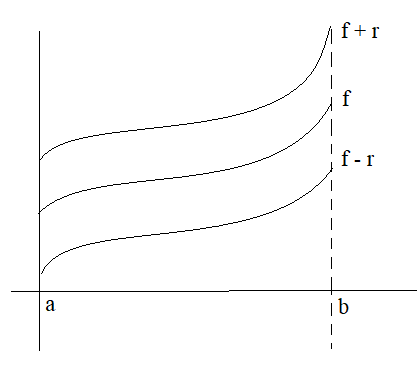
\includegraphics[width = 5cm]{lect2_1.png}
	$\overline{B}_r(f)$ состоит из тех непрерывных функций, графики которых содержатся в заштрихованном множестве.
\end{wrapfigure}

\textbf{Определение.} $(X, \rho)$ --- метрическое пространство, $A \subset X, x \in A.$

$x$ --- \textbf{внутренняя точка} $A \Leftrightarrow \exists \epsilon > 0: B_{\epsilon}(x) \subset A.$ 

$A$ называется \textbf{открытым} $\Leftrightarrow$ все его точки --- внутренние.

\textbf{Предложение 1}. Открытый шар $B_r(x)$ открыт.

\textbf{Доказательство.}

\begin{wrapfigure}{R}{0.3\textwidth}
	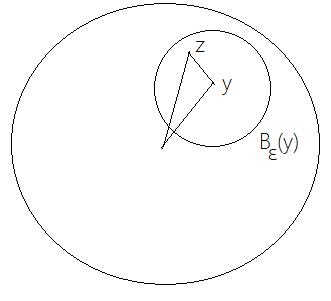
\includegraphics[width = 5cm]{lect2_2.png}
\end{wrapfigure}

Пусть $y \in B_r(x)$, т.е $\rho(y,x) < r.$

Положим $\epsilon = r - \rho(y,x).$

Покажем: $B_{\epsilon}(y) \subset B_r(x). (*)$

Пусть $z \in B_{\epsilon}(y).$

Неравенство треугольника: $\rho(z, x) \leqslant \rho(z, y) + \rho(y, x)< \epsilon + \rho(y, x) = r \Rightarrow z \in B_r(x) \Rightarrow \; (*)$ доказано $\Rightarrow B_r(x)$ открыто. 

\textbf{Предложение 2.}

(1) $\emptyset$ открыто;

(2) $X$ открыто;

(3) $\{U_i\}_{i \in I}$ --- семейство открытых множеств в $X \rightarrow \bigcup_{i \in I} U_i$ открыто.

(4) $U_1, U_2, \ldots, U_n \subset X$ открыты $\Rightarrow \bigcap^{n}_{i = 1} U_i$ открыто.

\textbf{Доказательство.} (1), (2) очевидны (из определения).

(3) $x \in \bigcup_{i \in I} U_i \Rightarrow \exists i_0 \in X: x \in U_{i_o} \Rightarrow \exists \epsilon > 0: B_{\epsilon}(x) \subset U_{i_0} \Rightarrow B_{\epsilon}(x) \subset \bigcup_{i \in I} U_i.$

(4) достаточно для $n = 2$

\begin{wrapfigure}{R}{0.3\textwidth}
	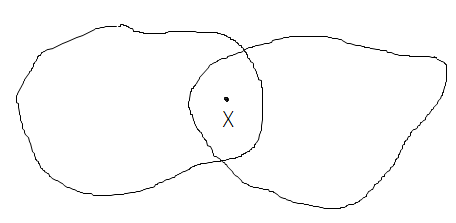
\includegraphics[width = 5cm]{lect2_3.png}
	$x \in U_1 \cap U_2$
\end{wrapfigure}

$\exists \epsilon_1 \epsilon_2 > 0: B_{\epsilon_1}(x) \subset U_1, B_{\epsilon_2} \subset U_2.$

Обозначим $\epsilon = \min\{\epsilon_1, \epsilon_2\} \Rightarrow B_{\epsilon}(x) \subset  U_1 \cap U_2.$

\section{Топологические пространства}

\textbf{Определение.} Пусть $X$ --- множество, $\tau \subset 2^{X}.$

\begin{wrapfigure}{R}{0.3\textwidth}
	Обозначение. $2^{X}$ --- множество всех подмножеств множества $X.$
\end{wrapfigure}

$\tau$ называется \textbf{топологией} на $X$, если

(1) $\emptyset \in \tau;$

(2) $X \in \tau;$

(3) $\{U_i\}_{i \in I}$ --- семейство множеств из $\tau \Rightarrow \bigcup_{i \in I} U_i \in \tau.$

(4) $U_1, \ldots, U_n \in \tau \Rightarrow \bigcap^n_{i = 1} U_i \in \tau.$

$\left(X, \tau \right)$ называется \textbf{топологическим пространством}.

Множества из $\tau$ называются \textbf{открытыми}.

\textbf{Наблюдение.} Из предложения 2: каждая метрика $\rho$ на множестве $X$ порождает топологию $\tau_{\rho}$ на $X.$

\textbf{Определение.} Топологическое пространство $(X, \tau)$ называется \textbf{метризуемым} $\Leftrightarrow \exists$ метрика $\rho: \; X\times X \to [0;\; +\infty): \tau_{\rho} = \tau.$

\textit{Замечение.} Если $\tau = \tau_{\rho},$ то такая $\rho$ не единственная! Например, $\tau_{\rho} = \tau_{2\rho}$

\textbf{Пример-упражнение.} Метрики $\rho_1, \rho_2, \rho_{\infty}$ на $\mathbb{K}^n$ (где $\mathbb{K} = \mathbb{R}$ либо $\mathbb{C}$) порождают одну и ту же топологию на $\mathbb{K}^n.$

\textbf{Пример 1.} Дискретная топология

$X$ -- $\forall$ множество, $\tau = 2^X.$

Рассмотрим $\rho: X \times X \to [0; \; +\infty), \quad \rho(x,y) = \begin{cases} 1, \text{если } \; x \neq y, \\ 0 \text{ иначе.} \end{cases}$

Заметим: $\tau = \tau_{\rho}.$

Действительно: $B_1(x) = {x} \Rightarrow {x}$ открыто в $\tau_{\rho} \; \forall x \in X \Rightarrow$ каждое $A \subset X$ открыто в $\tau_{\rho}$, так как $A = \bigcup_{x\in A} {x} \Rightarrow \tau_{\rho} = \tau$ --- дискретная топология (метризуема).

\textbf{Пример 2}. Антидискретная топология

$X$ - $\forall$ множество, $\tau = \{\emptyset, X\}.$

\textbf{Определение.} Пусть $\tau_1, \tau_2$ --- топологии на множестве $X.$

Говорят, что $\tau_1$ грубее $\tau_2$ ($\tau_2$ тоньше $\tau_1$), если $\tau_1 \subset \tau_2.$

Синонимы: грубее = слабее, тоньше = сильнее.

Дискретная топология --- самая тонкая, антидискретная --- самая грубая.

\textbf{Определение.} \textbf{Окрестность} точки $x$ в топологическом пространстве $X$ --- любое открытое множество $U \subset X$, содержащее $x.$

\textbf{Определение.} Топологическое пространство $X$ называется \textbf{хаусдорфовым} $\Leftrightarrow \forall x, y \in X, x \neq y, \exists$ окрестности $U \ni x, V \ni y: U \cap V = \emptyset.$

\textbf{Предложение.} Метризуемое топологическое пространство хаусдорфово.

\textit{Доказательство.} Пусть $(X, \rho)$ --- метрическое пространство, $x, y \in X, x \neq y$. Обозначим $a = \rho(x, y), \; a > 0.$

\begin{wrapfigure}{R}{0.3\textwidth}
	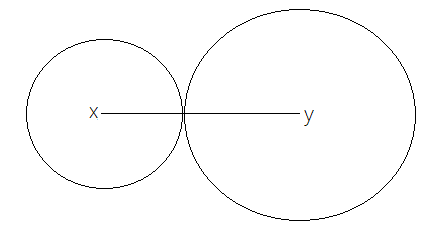
\includegraphics[width = 5cm]{lect2_4.png}
	Из неравенства треугольника: $B_{\frac{a}{2}}(x) \cap B_{\frac{a}{2}}(y) = \emptyset.$
\end{wrapfigure}

\textit{Следствие.} Антидискретная топология на множестве, содержащем более одного элемента, неметризуема (так как неухаусдорфова).

\textbf{Определение.} Пусть $X$ --- топологическое пространство.

Множество $F \subset X$ называется \textbf{замкнутым} $\Leftrightarrow X \backslash F$ открыто.

\textbf{Предложение.} Пусть $X$ --- топологическое пространство, $\tau' = \{ F \subset X: F \text{замкнуто}\}$. Тогда:

(1) $\emptyset \in \tau';$

(2) $x \in \tau';$

(3) $\{F_i\}$ - семейство множеств из $\tau' \Rightarrow \bigcap_{i \in I} F_i \in \tau';$

(4) $F_1, F_2, \ldots, F_n \in \tau' \Rightarrow \bigcup^n_{i = 1} F_i$ замкнуто.

\begin{wrapfigure}{R}{0.3\textwidth}
	Напоминание:
	
	$X \backslash \bigcap_{i \in I} F_i = \bigcup_{i \in I}\left( X \backslash F_i \right);$
	
	$X \backslash \bigcup_{i \in I} F_i = \bigcap_{i \in I}\left( X \backslash F_i \right).$
\end{wrapfigure}


\textbf{Наблюдение.} Если $X$ --- множество, $\tau' \subset 2^X$ удовлетворяет (1)-(4) из предложения $\Rightarrow \{X \backslash F \colon F \in \tau'\}$ --- топология на $X.$

\textbf{Пример.} Топология Зарисского

$X$ --- множество, $\mathbb{K} = \mathbb{R}$ или $\mathbb{C}$.

\textbf{Определение.} $A \subset \mathbb{K}^X$ - \textbf{подалгебра} в $\mathbb{K}^X,$ если

(1) $A$ --- векторное подпространство в $\mathbb{K}^X;$

(2) $1 \in A$ (где 1 -- функция, тождественно равная единице);

(3) $f, g \in A \Rightarrow fg \in A$ ($fg$ --- поточечное произведение $f$ и $g$).

Зафиксируем какую-либо подалгебру $A \subset \mathbb{K}^X.$

$\forall S \subset A$ обозначим $V(S) = \{ x \in X: \; \forall f \in S \; f(x) = 0 \}$ 

\textit{Упражнение.} На $X$ существует топология, в которой $F \subset X$ замкнуто $\Leftrightarrow F = V(S)$ для некоторого $S \subset A$. \\Она называется \textbf{топологией Зарисского.}

Важный частный случай: $X = \mathbb{K}^n, \; A = \mathbb{K}[t_1, \ldots, t_n].$

\textbf{Упражнение.} Описать топологию Зарисского в явном виде для следующих случаев:

(1) $X$ --- любое множество, $A = \mathbb{K}^X;$

(2) $X = \mathbb{K}, \; A = \mathbb{K}[t];$

(3) $X = [a, b] \subset \mathbb{R}, \; A = C[a,b].$

\section{Открытое множество в метрическом пространстве}

$(X, \rho)$ --- метрическое пространство, $x \in X, r \geqslant 0$.

\textbf{Определение.} Открытый шар с центром в $x$ радиуса $r$ --- это 
$B_r(x) = \{ y \in X: \rho(y, x) < r\}$ --- r-окрестность x. 

\textit{Замкнутый шар} с центром в $x$ радиуса $r$ --- это
$\overline{B}_r(x) = \{ y\in X: \rho(y, x) \leqslant r\}.$

\textbf{Пример.} $x = \mathbb{R} \Rightarrow B_r(x) = (x - r, x + r); \quad \overline{B}_r(x) = [x - r, x+r].$

\textbf{Упражнение.} Нарисовать $B_1(o)$ на $(\mathbb{R}^2, \rho_p)$ для $p = 1, p = 2, p = \infty$ (для $p = 2$ --- круг, для $p = 3$ --- шар, как в школе).

\textbf{Пример.} $X = C[a,b]$ с равномерной метрикой.

\begin{wrapfigure}{R}{0.3\textwidth}
	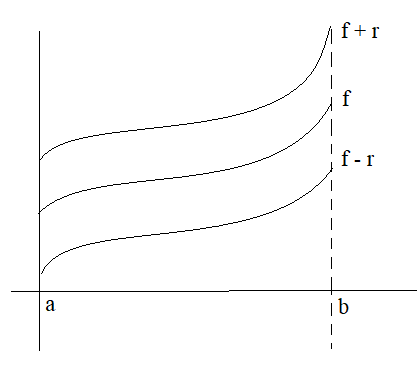
\includegraphics[width = 5cm]{lect2_1.png}
	$\overline{B}_r(f)$ состоит из тех непрерывных функций, графики которых содержатся в заштрихованном множестве.
\end{wrapfigure}

\textbf{Определение.} $(X, \rho)$ --- метрическое пространство, $A \subset X, x \in A.$
$x$ --- \textbf{внутренняя точка} $A \Leftrightarrow \exists \epsilon > 0: B_{\epsilon}(x) \subset A.$ 

$A$ называется \textbf{открытым} $\Leftrightarrow$ все его точки --- внутренние.

\textbf{Предложение 1}. Открытый шар $B_r(x)$ открыт.

\textbf{Доказательство.}

\begin{wrapfigure}{R}{0.3\textwidth}
	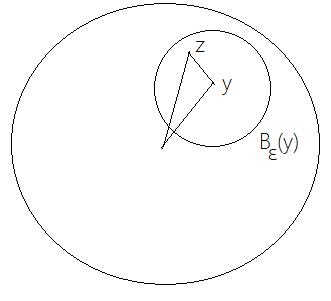
\includegraphics[width = 5cm]{lect2_2.png}
\end{wrapfigure}

Пусть $y \in B_r(x)$, т.е $\rho(y,x) < r.$

Положим $\epsilon = r - \rho(y,x).$

Покажем: $B_{\epsilon}(y) \subset B_r(x). (*)$

Пусть $z \in B_{\epsilon}(y).$

Неравенство треугольника: $\rho(z, x) \leqslant \rho(z, y) + \rho(y, x)< \epsilon + \rho(y, x) = r \Rightarrow z \in B_r(x) \Rightarrow \; (*)$ доказано $\Rightarrow B_r(x)$ открыто. 

\textbf{Предложение 2.}

(1) $\emptyset$ открыто;

(2) $X$ открыто;

(3) $\{U_i\}_{i \in I}$ --- семейство открытых множеств в $X \rightarrow \bigcup_{i \in I} U_i$ открыто.

(4) $U_1, U_2, \ldots, U_n \subset X$ открыты $\Rightarrow \bigcap^{n}_{i = 1} U_i$ открыто.

\textbf{Доказательство.} (1), (2) очевидны (из определения).

(3) $x \in \bigcup_{i \in I} U_i \Rightarrow \exists i_0 \in X: x \in U_{i_o} \Rightarrow \exists \epsilon > 0: B_{\epsilon}(x) \subset U_{i_0} \Rightarrow B_{\epsilon}(x) \subset \bigcup_{i \in I} U_i.$

(4) достаточно для $n = 2$

\begin{wrapfigure}{R}{0.3\textwidth}
	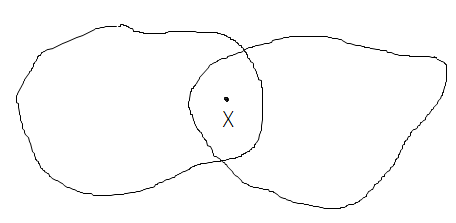
\includegraphics[width = 5cm]{lect2_3.png}
	$x \in U_1 \cap U_2$
\end{wrapfigure}

$\exists \epsilon_1 \epsilon_2 > 0: B_{\epsilon_1}(x) \subset U_1, B_{\epsilon_2} \subset U_2.$

Обозначим $\epsilon = \min\{\epsilon_1, \epsilon_2\} \Rightarrow B_{\epsilon}(x) \subset  U_1 \cap U_2.$

\section{Топологические пространства}

\textbf{Определение.} Пусть $X$ --- множество, $\tau \subset 2^{X}.$

\begin{wrapfigure}{R}{0.3\textwidth}
	Обозначение. $2^{X}$ --- множество всех подмножеств множества $X.$
\end{wrapfigure}

$\tau$ называется \textbf{топологией} на $X$, если

(1) $\emptyset \in \tau;$

(2) $X \in \tau;$

(3) $\{U_i\}_{i \in I}$ --- семейство множеств из $\tau \Rightarrow \bigcup_{i \in I} U_i \in \tau.$

(4) $U_1, \ldots, U_n \in \tau \Rightarrow \bigcap^n_{i = 1} U_i \in \tau.$

$\left(X, \tau \right)$ называется \textbf{топологическим пространством}.

Множества из $\tau$ называются \textbf{открытыми}.

\textbf{Наблюдение.} Из предложения 2: каждая метрика $\rho$ на множестве $X$ порождает топологию $\tau_{\rho}$ на $X.$

\textbf{Определение.} Топологическое пространство $(X, \tau)$ называется \textbf{метризуемым} $\Leftrightarrow \exists$ метрика $\rho: \; X\times X \to [0;\; +\infty): \tau_{\rho} = \tau.$

\textit{Замечение.} Если $\tau = \tau_{\rho},$ то такая $\rho$ не единственная! Например, $\tau_{\rho} = \tau_{2\rho}$

\textbf{Пример-упражнение.} Метрики $\rho_1, \rho_2, \rho_{\infty}$ на $\mathbb{K}^n$ (где $\mathbb{K} = \mathbb{R}$ либо $\mathbb{C}$) порождают одну и ту же топологию на $\mathbb{K}^n.$

\textbf{Пример 1.} Дискретная топология

$X$ -- $\forall$ множество, $\tau = 2^X.$

Рассмотрим $\rho: X \times X \to [0; \; +\infty), \quad \rho(x,y) = \begin{cases} 1, \text{если } \; x \neq y, \\ 0 \text{ иначе.} \end{cases}$

Заметим: $\tau = \tau_{\rho}.$

Действительно: $B_1(x) = {x} \Rightarrow {x}$ открыто в $\tau_{\rho} \; \forall x \in X \Rightarrow$ каждое $A \subset X$ открыто в $\tau_{\rho}$, так как $A = \bigcup_{x\in A} {x} \Rightarrow \tau_{\rho} = \tau$ --- дискретная топология (метризуема).

\textbf{Пример 2}. Антидискретная топология

$X$ - $\forall$ множество, $\tau = \{\emptyset, X\}.$

\textbf{Определение.} Пусть $\tau_1, \tau_2$ --- топологии на множестве $X.$

Говорят, что $\tau_1$ грубее $\tau_2$ ($\tau_2$ тоньше $\tau_1$), если $\tau_1 \subset \tau_2.$

Синонимы: грубее = слабее, тоньше = сильнее.

Дискретная топология --- самая тонкая, антидискретная --- самая грубая.

\textbf{Определение.} \textbf{Окрестность} точки $x$ в топологическом пространстве $X$ --- любое открытое множество $U \subset X$, содержащее $x.$

\textbf{Определение.} Топологическое пространство $X$ называется \textbf{хаусдорфовым} $\Leftrightarrow \forall x, y \in X, x \neq y, \exists$ окрестности $U \ni x, V \ni y: U \cap V = \emptyset.$

\textbf{Предложение.} Метризуемое топологическое пространство хаусдорфово.

\textit{Доказательство.} Пусть $(X, \rho)$ --- метрическое пространство, $x, y \in X, x \neq y$. Обозначим $a = \rho(x, y), \; a > 0.$

\begin{wrapfigure}{R}{0.3\textwidth}
	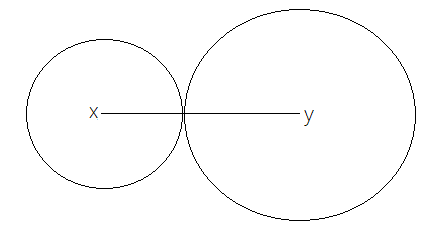
\includegraphics[width = 5cm]{lect2_4.png}
	Из неравенства треугольника: $B_{\frac{a}{2}}(x) \cap B_{\frac{a}{2}}(y) = \emptyset.$
\end{wrapfigure}

\textit{Следствие.} Антидискретная топология на множестве, содержащем более одного элемента, неметризуема (так как неухаусдорфова).

\textbf{Определение.} Пусть $X$ --- топологическое пространство.

Множество $F \subset X$ называется \textbf{замкнутым} $\Leftrightarrow X \backslash F$ открыто.

\textbf{Предложение.} Пусть $X$ --- топологическое пространство, $\tau' = \{ F \subset X: F \text{замкнуто}\}$. Тогда:

(1) $\emptyset \in \tau';$

(2) $x \in \tau';$

(3) $\{F_i\}$ - семейство множеств из $\tau' \Rightarrow \bigcap_{i \in I} F_i \in \tau';$

(4) $F_1, F_2, \ldots, F_n \in \tau' \Rightarrow \bigcup^n_{i = 1} F_i$ замкнуто.

\begin{wrapfigure}{R}{0.3\textwidth}
	Напоминание:
	
	$X \backslash \bigcap_{i \in I} F_i = \bigcup_{i \in I}\left( X \backslash F_i \right);$
	
	$X \backslash \bigcup_{i \in I} F_i = \bigcap_{i \in I}\left( X \backslash F_i \right).$
\end{wrapfigure}


\textbf{Наблюдение.} Если $X$ --- множество, $\tau' \subset 2^X$ удовлетворяет (1)-(4) из предложения $\Rightarrow \{X \backslash F \colon F \in \tau'\}$ --- топология на $X.$

\textbf{Пример.} Топология Зарисского

$X$ --- множество, $\mathbb{K} = \mathbb{R}$ или $\mathbb{C}$.

\textbf{Определение.} $A \subset \mathbb{K}^X$ - \textbf{подалгебра} в $\mathbb{K}^X,$ если

(1) $A$ --- векторное подпространство в $\mathbb{K}^X;$

(2) $1 \in A$ (где 1 -- функция, тождественно равная единице);

(3) $f, g \in A \Rightarrow fg \in A$ ($fg$ --- поточечное произведение $f$ и $g$).

Зафиксируем какую-либо подалгебру $A \subset \mathbb{K}^X.$

$\forall S \subset A$ обозначим $V(S) = \{ x \in X: \; \forall f \in S \; f(x) = 0 \}$ 

\textit{Упражнение.} На $X$ существует топология, в которой $F \subset X$ замкнуто $\Leftrightarrow F = V(S)$ для некоторого $S \subset A$. \\Она называется \textbf{топологией Зарисского.}

Важный частный случай: $X = \mathbb{K}^n, \; A = \mathbb{K}[t_1, \ldots, t_n].$

\textbf{Упражнение.} Описать топологию Зарисского в явном виде для следующих случаев:

(1) $X$ --- любое множество, $A = \mathbb{K}^X;$

(2) $X = \mathbb{K}, \; A = \mathbb{K}[t];$

(3) $X = [a, b] \subset \mathbb{R}, \; A = C[a,b].$

\section{База и предбаза топологии}

\textbf{Лемма.} X --- множество, $\beta \subset 2^{X}.$ Следующие свойства множества $A \subset X$ эквиваленты: 

\begin{wrapfigure}{R}{0.3\textwidth}
	
	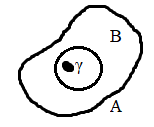
\includegraphics[width = 5cm]{lect3_1.png}
	
	$\gamma \subset 2^X$
	
	Обозначение: $\bigcup_{C \in \gamma} C = \cup \gamma$
\end{wrapfigure}

$(1) \; \exists \gamma \subset \beta$ т.ч. $A = \cup \gamma;$

$(2) \; \forall x \in A \; \exists B \in \beta$ т.ч. $x \in B \subset A.$ 

\textbf{Доказательство.} $(1) \Rightarrow (2).$ Пусть $A = \cup \gamma, \gamma \subset \beta, x \in A \Rightarrow \exists B \in \gamma: x \in B \Rightarrow$ B удовлетворяет (2). 

$(2) \Rightarrow \forall x \in A \; \exists B_{1} \in \beta: x \in B_{1} \subset A \Rightarrow \gamma = \{B_{x}: x \in A\}$ удовлетворяет (1). 

\textbf{Определение.} $(x, \tau)$ --- топологическое пространство. 

$(1) \; \beta \in \tau$ --- база $\tau$ (или база $(X, \tau)) \Leftrightarrow$ каждое $U \in \tau$ является объединением некоторого подсемейства в $\beta \Leftrightarrow \forall U \in \tau \; \forall x \in U \; \exists B \in \beta$ т.ч. $x \in B \subset U.$ 

$(2) \sigma \subset \tau$ --- предбаза $\tau$ (предбаза $(x, \tau)$ --- из леммы) $\Leftrightarrow$ семейство $\{U_{1} \cap \ldots \cap U_{n}: U_{i} \in \sigma, \; n \in \mathbb{N}\}$ --- база $\tau.$ 

\textbf{Пример.} $(x, \rho)$ --- метрическое пространство $\Leftrightarrow \{B_{r}(x): x \in X, r > 0\}$ --- база $\tau_{p}.$

\textbf{Пример.} $X = \mathbb{R}, \; \sigma = \{(-\infty, b); (a, +\infty): a, b \in \mathbb{R}\}$ --- предбаза $\mathbb{R},$ но не база. 

\textbf{Предложение.} X --- множество, $\beta, \sigma \subset 2^{X}.$

(1) На X $\exists$ топология с базой $\beta \Leftrightarrow$ $\begin{cases} 
(a) \cup \beta = X \\
(b) \forall B_{1}, B_{2} \in \beta \; \forall x \in B_{1} \cap B_{2} \; \exists B_{3} \in \beta: \\ x \in B_{3} \subset B_{1} \cap B_{2}.
\end{cases}$

(2) На X $\exists$ топология с предбазой $\sigma \Leftrightarrow \cup \sigma = X.$ 

\begin{wrapfigure}{R}{0.3\textwidth}
	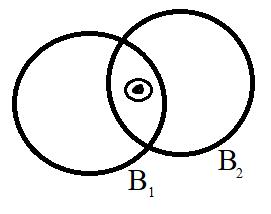
\includegraphics[width = 5cm]{lect3_2.png}
\end{wrapfigure}

\textbf{Доказательство.} (1) $(\Leftarrow)$ следует из открытости X и $B_{1} \cap B_{2}.$ 

$\Rightarrow$ Обозначим $\tau = \{\cup \gamma: \gamma \in \beta\}.$ Покажем, что $\tau$ --- топология на X. 

$\emptyset = \cup \emptyset \in \tau; \; X = \cup \beta \in \tau;$ объединение множеств из $\tau$ принадлежит $\tau.$

Пусть $U_{1}, U_{2} \in \tau.$ Хотим: $U_{1} \cap U_{2} \in \tau.$

Пусть $x \in U_{1} \cap U_{2} \xRightarrow{\text{из леммы}}$ $\exists B_{1}, B_{2} \in \beta$ т.ч. $x \in B_{k} \subset U_{k} (k = 1, 2) \Rightarrow x \in B_{1} \cap B_{2} \Rightarrow^{(b)} \Rightarrow \exists B_{3} \in \beta$ т.ч. $x \in B_{3} \subset B_{1} \cap B_{2} \subset U_{1} \cap U_{2} \xRightarrow{\text{из леммы}} U_{1} \cap U_{2} \in \tau \Rightarrow \tau$ --- топология на X, $\beta$ --- ее база. 

(2) $(\Rightarrow)$ из открытости X. 

$(\Leftarrow)$ cемейство $\{U_{1} \cap \ldots \cap U_{n}: U_{i} \in \sigma, n \in \mathbb{B}\}$ удовлетворяет (a), (b) $\Rightarrow$ оно --- база топологии, а $\sigma$ --- ее предбаза. 

\textbf{Пример.} Топология поточечной сходимости

\begin{wrapfigure}{R}{0.3\textwidth}
	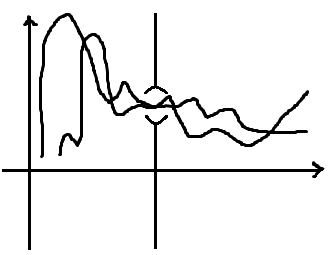
\includegraphics[width = 5cm]{lect3_3.png}
\end{wrapfigure}

Пусть $\mathbb{K} = \mathbb{R}$ или $\mathbb{C}, \; S \subset \mathbb{K}^{X},$ где $X - \forall$ множество) 

$\forall x \in X, \forall$ интервала $I \subset \mathbb{R}$ обозначается $G(x, I) = \{f \in S: f(x) \in I\}.$ 

Семейство $\{G(x, I): x \in X, I \subset R$ --- интервал (для $\mathbb{K} = \mathbb{C}$ --- открытый круг)\} является предбазой некоторой топологии на S. Она называется \textbf{топологией поточечной сходимости} на S. 

\section{Сходимость последовательностей в топологическом пространстве}

(Окрестность точки --- это любое открытое множество, содержащее эту точку)

X --- топологическое прространство, $x \in X, (x_{n})$ --- последовательность в X. 

\textbf{Опредедение.} $(x_{n})$ сходится к $x$ ($x$ является пределом $(x_{n}) \Leftrightarrow \forall$ окрестности $U \ni x \; \exists N \in \mathbb{N} \forall n \geqslant N \; x_{n} \in U.$

\textbf{Обозначение.} $x_{n} \to x (n \to \infty),$ или $x = \lim_{n \to \infty} x_{n}.$ 

\textbf{Определение.} (1) Семейство $\beta_{x}$ окрестностей точки $x \in X$ --- база окрестностей x (база в x) $\Rightarrow \forall$ окрестности $U \in$ (знак наоборот) $\exists V \in \beta_{x}, V \subset U.$

(2) Семейство $\sigma_{1}$ окрестностей точки $x \in X$ --- предбаза окрестностей x (предбаза в x). 

$\Leftrightarrow \{U_{1} \cap \ldots \cap\ldots U_{n}: U_{i} \in \sigma_{x}, n \in \mathbb{N}\}$ --- база в x. 

\textbf{Пример.} $(x, \rho)$ --- метрическое пространство. 

\begin{wrapfigure}{R}{0.3\textwidth}
	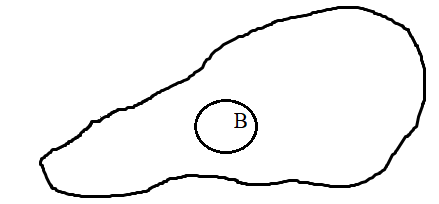
\includegraphics[width = 5cm]{lect3_4.png}
\end{wrapfigure}

$\{B_{r}(x): r > 0\}$ --- база в x. 

$\{B_{\frac{1}{n}}(x): n \in \mathbb{N}\}$ --- тоже (важный пример, запомнить.)

\textbf{Предложение.} X --- топологическое пространство, $x \in X, \sigma_{x}$ --- предбаза в x, $(x_{n})$ --- последовательность в X.

$x_{n} \to x \; (n \to \infty) \Leftrightarrow \forall V \in \sigma_{x} \exists N \in \mathbb{N} \forall n \geqslant N \; x_{n} \in V.$

\textbf{Доказательство.} $(\Leftarrow)$ Пусть U --- окрестность x $\Rightarrow \exists V{1}, \ldots, V_{p} \in \sigma_{x}$ т.ч. $V_{1} \cap \ldots \cap V_{p} \subset U.$ 

$\exists N_{1}, \ldots, N_{p}$ т.ч. $\forall n \geqslant N_{i} \; x_{n} \in V_{i} (i = 1, \ldots, p).$

Обозначим $N = \max_{1 \leqslant i \leqslant n} N_{i} \Rightarrow \forall n \geqslant N \; x_{n} \in V_{1} \cap \ldots \cap V_{p} \subset U.$ 


\textbf{Следствие.} $(x, \rho)$ --- метрическое пространство, $x \in X, (x_{n})$ --- последовательность в X. Следующие утверждения эквивалентны: 

$(1) \; x_{n} \to x$

$(2) \; \forall$ открытого щара V с центром в x $\exists N \in \mathbb{N} \; \forall n \geqslant N\; x_{n} \in V$

$(3) \forall \epsilon > 0 \exists N \in \mathbb{N} \; \forall n \geqslant N \rho(x_{n}, x) < \epsilon.$

$(4) \rho(x_{n}, x) \to 0$

\textbf{Предложение.} X --- хаусдорфово топологического пространство, $(x_{n})$ --- последовательность в X, $x_{n} \to x \in X, \; x_{n} \to y \in X \Rightarrow x = y.$ 

\textbf{Доказательство.} Пусть $x \neq y \Rightarrow \exists$ окрестности $U \ni x$, $V \ni y, \; U \cap V = \emptyset.$

Из $\exists N_{1}$ т.ч. $\forall n \geqslant N_{1} x_{n} \in U$ и $\exists N_{2}$ т.ч. $\forall n \geqslant N_{2} \; x_{n} \in V$ следует, что $x_{n} \in U \cap V \; \forall n \geqslant \max{N_{1}, N_{2}}$ --- противоречие. 

\textbf{Пример.} X --- антидискретное пространство. Каждая последовательность в X сходится к каждой точке $x \in X.$ 

\textbf{Пример.} X --- дискретное топологическое пространство $x_{n} \to x \Leftrightarrow \exists N \in \mathbb{N} \; \forall n \geqslant N x_{n} = x.$ 

Действительно: $(\Rightarrow) \; {x}$ --- окрестность x. Далее см. определение сходимости. 

\textbf{Пример-упражнение.} $\mathbb{K} = \mathbb{R}$ или $\mathbb{c}, X$ --- множество, $S \subset \mathbb{K}^{X}.$

Пусть $f_{n} \to F$ в $S$ с топологией поточечной сходимости $\Leftrightarrow \forall x \in X \; f_{n}(x) \to f(x).$

\section{Замыкание, внутренность, граница} 

X --- топологическое пространство, $A \subset X.$ 

\textbf{Определение.} Замыкание A --- множество $\overline{A} = \cap\{F \subset X: F$ замкнуто, $A \subset F\}.$ 

\textbf{Наблюдение.} $\overline{A}$ --- наименьшее замкнутое множество, содержащее A. В частности, если A замкнуто, то $A = \overline{A}.$ 

\textbf{Предложение.} $(1) A \subset B \subset X \Rightarrow \overline{A} \subset \overline{B};$

$(2) \overline{\overline{A}} = \overline{A};$ 

$(3) \overline{A \cup B} = \overline{A} \cup \overline{B}.$

\textbf{Доказательство.} (1) из определения, (2) из наблюдения, (3) $A \subset A \cup B \xRightarrow{(1)} \overline{А} \subset \overline{A \cup B}.$ Аналогично $\overline{B} \subset \overline{A \cup B} \Rightarrow \overline{A} \cup \overline{B} \subset \overline{A \cup B}.$

$A \cup B \subset \overline{A} \cup \overline{B} \xRightarrow{(1)} \overline{A \cup B} \subset \overline{\overline{\overline{А} \cup \overline{B}}} = \overline{A} \cup \overline{B},$ так как $\overline{A} \cup \overline{B}$ замкнуто.

\textbf{Предложение.} $x \in \overline{A} \Leftrightarrow$ окрестности $U \ni x, \; U \cap A \neq \emptyset.$ 

\textbf{Доказательство.} $x \notin \overline{A} \Leftrightarrow \exists$ замкнутое $F \subset X$ т.ч. $F \supset A, \; x \notin F \; \xLeftrightarrow{U = X\backslash F} \exists x \in U$ и $\exists$ открытое $U \subset X$ т.ч. $U \cap A = \emptyset \Leftrightarrow \exists$ окрестность $U \ni x, \; U \cap A = \emptyset.$

\textbf{Определение.} X --- топологическое пространство, $A \subset X.$ Тогда $x \in X$ --- \textbf{предельная точка} A $\Leftrightarrow \; x \in \overline{A\backslash{\{x\}}} \xLeftrightarrow{\text{предложение}}$ в каждой окрестности x есть точки из A, отличные от x. 

\textbf{Обозначение.} $A' = \{x \in X | x$ --- предельная точка A\} --- производное множество множества A.

Из предложения $\overline{A} = A \cup A'.$ В частности: A замкнуто $\Leftrightarrow A' \subset A.$ 

\textbf{Определение.} $x \in A$ --- \textbf{изолированная точка} A $\Leftrightarrow x \in A \backslash A' \Leftrightarrow \exists$ окрестность $U \ni x$ т.ч. $U \cap A = \{x\}.$ 

$\overline{A} = A' \sqcup$ {изолированные точки A}.

\subsection{Внутренность}

X --- топологическое пространство, $A \subset X.$ 

\textbf{Определение.} \textbf{Внутренность} A --- это Int(A) = $\bigcup \{U \subset X: U$ открыто, $U \subset A\}.$ 

\textbf{Наблюдение.} (1) Int A --- наибольшее открытое множество, содержащееся в A. В частности: A открытое $\Leftrightarrow$ A = Int A. 

$\quad \quad \quad$ Если $(x, \rho)$ --- метрическое пространство, то $x \in Int A \Leftrightarrow \exists \epsilon > 0$ т.ч. $B_{\epsilon}(x) \subset.$ 

\textbf{Упражнение.} Int A = $X \backslash \overline{(X \backslash A)}; \quad \overline{A} = X \backslash Int(X \backslash A).$

(в рамочке) Int A $subset A \subset \overline{A}.$ 

\textbf{Определение.} \textbf{Граница} A --- это $\delta A = \overline{A} \backslash$ Int A. 

\textbf{Наблюдение.} $x \in \delta A \Leftrightarrow \forall$ окрестностей $U \ni x \; U\cap A \neq \emptyset, \; U \cap (X \backslash A) \neq \emptyset.$

\textbf{Примечание 1.} $X = \mathbb{R}, A = \mathbb{Z} \Rightarrow \overline{A} = \mathbb{Z},$ Int $A = \emptyset, \; \delta A = A = \mathbb{Z},$ все точки A изолированы, $A' = \emptyset.$ 

\begin{wrapfigure}{R}{0.3\textwidth}
	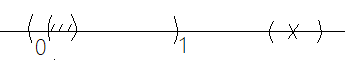
\includegraphics[width = 5cm]{lect4_1.png}
\end{wrapfigure}

\textbf{Примечание 2.} $X = \mathbb{R}, A = (0, 1) \Rightarrow \overline{A} = [0, 1],$ Int A = A = (0, 1), $\delta A = \{0, 1\},$ изолированных точек нет, A' = [0, 1].

\begin{wrapfigure}{R}{0.3\textwidth}
	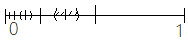
\includegraphics[width = 5cm]{lect4_2.png}
\end{wrapfigure}

\textbf{Примечание 3.} $X = \mathbb{R}, A = \{\dfrac{1}{n}: n \in \mathbb{N}\} \cup \{0\ \Rightarrow \overline{A} = A$ (т.к. $\mathbb{R} \backslash A = (-\infty, 0) \cup (1, +\infty) \cup (\bigcup^{\infty}_{n = 1} (\dfrac{1}{n + 1}, \dfrac{1}{n})).$ Int $A = \emptyset, \; \delta A = A,$ \{изолированные точки A\} = $\{\dfrac{1}{n}: n \in \mathbb{N}\}; \{0\} = A'.$ 

\textbf{Определение.} X --- топологическое пространство. Множество $A \subset X$ \textbf{плотно} в X (= \textbf{всюду плотно} в X) $\Leftrightarrow \overline{A} = X.$ 

\textbf{Наблюдение.} A плотно в X $\Leftrightarrow \forall x \in X \forall$ окрестности $U \ni x \; U \cap A \neq \emptyset \Leftrightarrow \forall$ непустого открытого $U \subset X \; U \cap A \neq \emptyset.$ 

\textbf{Определение.} X \textbf{сепарабельно} $\Leftrightarrow \; \exists$ не более чем счетное плотное подмножество в X. 

\textbf{Пример 1.} Дискретное пространство сепарабельно $\Leftrightarrow$ оно само не более чем счетно. 

\textbf{Пример 2.} Антидискретное пространство сепарабельно (каждое непустое подмножество плотно). 

\textbf{Пример 3.} $\mathbb{R}$ сепарабельно (т.к. $\mathbb{Q}$ плотно в $\mathbb{R}$). 

\textbf{Пример-упражнение 4.} $\mathbb{R}^n, \mathbb{C}^n, l^{1}, l^{2}$ сепарабельны, $l^{\infty}$ несепарабельно. 

\section{Аксиомы счетности}

X --- топологическое пространство. 

\textbf{Определение.} (1) X удовлетворяет \textbf{1-ой аксиоме счетности} $\Leftrightarrow \forall x \in X \exists$ не более чем счетная база окрестностей x.

$\quad \quad \quad \quad$ (2) X удовлетворяет \textbf{2-ой аксиоме счетности} (является пространством со \textbf{счетной базой}) $\Leftrightarrow \exists$ не более чем счетная база топологии на X. 

\textbf{Предложение.} X удовлетворяет 2-ой аксиоме счетности $\Rightarrow$ X удовлетворяет 1-ой аксиоме счетности. 

\textbf{Доказательство.} Пусть $\beta$ --- не более чем счетная база топологии на X. $x \in X;$ тогда $\{U \in \beta: \; U \ni x\}$ --- база окрестностей x. 

\textbf{Пример 1.} X --- метризуемо $\Rightarrow$ X удовлетворяет 1-ой аксиоме счетности. Действительно, $\forall x \in X \; \{B_{\frac{1}{n}}(x): \; n \in \mathbb{N}\}$ --- база окрестностей x. 

\textbf{Определение.} Семейство $\beta_{x}$ окрестностей точки $x \in X$ --- \textbf{база окрестностей x} $\Leftrightarrow \forall$ окрестности $U \ni x \; \exists V \in \beta_{x}, \; V \subset U.$

\textbf{Пример 2.} Дискретное пространство X удовлетворяет 1-ой аксиоме счетности. Оно удовлетворяет 2-ой аксиоме счетности $\Leftrightarrow$ оно не более чем счетно. 

\textbf{Пример 3.} $\mathbb{R}$ удовлетворяет 2-ой аксиоме счетности. А именно, $\{(a, b): a < b, a, b \in \mathbb{Q}\}$ --- база $\mathbb{R}.$ Действительно, $\forall c, d \in \mathbb{R}, \; c < d,$ выполнено $(c, d) = \bigcup\{(a, b): a, b \in \mathbb{Q}, \; c < a < b < d\}$ --- в силу плотности $\mathbb{Q}$ в $\mathbb{R}.$ 

\textbf{Предложение.} Топологическое пространство со счетной базой сепарабельно. 

\textbf{Доказательство.} $\{U_{n}: \; n \in \mathbb{N}\}$ --- счетная база в X; $U_{n} \neq \emptyset \; \forall n$ (если пусто, можно выкинуть и ничего не потерять). $\forall n \in \mathbb{N}$ выберем $x_{n} \in U_{n} \Rightarrow \{x_{n}: \; n \in \mathbb{N}\}$ плотно в X. 

\textbf{Упражнение.} Для метризуемых пространств: счетная база $\Leftrightarrow$ сепарабельность. В частности: $\mathbb{R}^n, \mathbb{C}^n, l^{1}, l^{2}$ --- со счетной базой. 

\textbf{Лемма.} Пусть X --- топологическое пространство, удовлетворяющее 1-й аксиоме счетности. Тогда $\forall x \in X\; \exists$ база окрестностей $\{U_{n}: n \in \mathbb{N}\}$ точки x, т.ч. $U_{n} \supset U_{n + 1} \; \forall n.$

\textbf{Доказательство.} Пусть $\{V_{n}: \; n \in \mathbb{N}\}$ --- база окрестностей x; обозначим $U_{n} = V_{1} \cap ... \cap V_{n} \Rightarrow \{U_{n}: \; n \in \mathbb{N}\}$ --- искомая. 

\textbf{Предложение.} X --- топологическое пространство, $A \subset X, \; x \in X.$ 

(1) Если $\exists$ последовательность $(x_{n})$ в A т.ч. $x_{n} \to x \; \Rightarrow \; x \in \overline{A};$ 

(2) Если X удовлетворяет 1-й аксиоме счетности, то верно и обратное. 

\textbf{Доказательство.} $(1) \Rightarrow (2).$ Пусть U --- окрестность x. $\Rightarrow \; \exists n \in \mathbb{N}$ т.ч. $x_{n} \in U \Rightarrow U \cap A \neq \emptyset \Rightarrow x \in \overline{A}.$ 

$(2) \Rightarrow (1).$ Пусть $x \in \overline{A}$ и пусть $\{U_{n}: \; n \in \mathbb{N}\}$ --- база окрестностей x т.ч. $U_{n + 1} \subset U_{n} \; \forall n$ выберем $\forall x_{n} \in U_{n} \cap A.$ Покажем: $x_{n} \to x.$ 

Пусть U --- окрестность x. $\exists N \in N$ т.ч. $U_{N} \subset U \; \Rightarrow \forall n \neq N \; x_{n} \in U_{n} \subset U_{N} \subset U \Rightarrow x_{n} \to x.$

\section{Непрерывные отображения} 

\begin{wrapfigure}{R}{0.3\textwidth}
	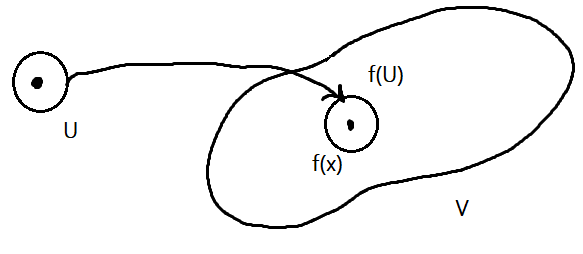
\includegraphics[width = 5cm]{lect4_3.png}
\end{wrapfigure}

\textbf{Определение.} X, Y --- топологические пространства, $f: \; X \to Y, \; x \in X.$ 

f \textbf{непрерывно} в x $\Leftrightarrow \; \forall$ окрестности $V \ni f(x) \; \exists$ окрестность $U \ni x$ т.ч. $f(U) \subset V.$ 

f \textbf{непрерывно} $\Leftrightarrow$ оно непрерывно в каждой $x \in X.$ 

\textbf{Предложение.} Пусть $f: X \to Y$ --- отображение топологических пространств, $x \in X, \; y = f(x).$ 

$\beta_{x}$ --- база топологии x, $\sigma_{y}$ --- предбаза окрестностей y. Тогда: 

f непрерывно в x $\Leftrightarrow \; \forall V \in \sigma_{y} \exists$ окрестность $W \ni x$ т.ч. $f(w) \subset V; \; \exists V \in \beta_{x}$ т.ч. $U \subset W \Rightarrow f(x) \subset V.$ 

$(\Leftarrow)$ Пусть V --- окрестность y. $\exists V_{1}, ..., V_{p} \in \sigma_{y}$ т.ч. $V_{1} \cap ... \cap V_{p} \subset V; \; \forall i = 1, ..., p \; \exists U_{i} \in \beta_{x}$ т.ч. $f(V_{i}) \subset V_{i} \; \ f(U_{1} \cap ... \cap U_{p}) \subset V.$

\textbf{Следствие.} $(X, \rho_{X}), \; (Y, \rho_{Y})$ --- метрические пространства, $x \in X.$ 

Отображение $f: X \to Y$ непрерывно в x $\Leftrightarrow \; \forall \epsilon > 0 \; \exists \delta > 0$ т.ч. $\forall x' \in X,$ удовлетворяющей $\rho_{X}(x, x') < \delta,$ выполнено $\rho_{Y}(f(x), f(x')) < \epsilon.$ 

\textbf{Доказательство.} Применить предложение к базам окрестностей x и f(x), состоящим из открытых шаров с центрами x и y. 

\textbf{Теорема.} X, Y --- топологические пространства, $f: X \to Y$ --- отображение. Следующие утверждения эквивалентны: 

(1) f непрерывно; 

Часто берут в качестве определения непрерывности отображения: $(2)!!! \; \forall$ открытых $V \subset Y \; f^{-1}(V)$ открыты в X; 

(3) $\forall$ замкнуто $B \subset Y \; f^{-1}(B)$ замкнуто в X; 

(4) $\forall A \subset X \; f(\overline{A}) \subset \overline{f(A)}.$

\textbf{Доказательство.} $(1) \Rightarrow (2).$ Пусть $V \subset Y$ --- открыто. $\forall x \in f^{-1}(V) \; \exists$ окрестность $U_{x} \ni x$ т.ч. $f(U_{x}) \subset V \Rightarrow U_{x} \subset f^{-1} \Rightarrow \bigcap_{x \in f^{-1}}
U_{x} = f^{-1}(V) \Rightarrow f^{-1}(V)$ открыто. 

$(2) \Leftrightarrow (3)$ --- следствие из равенства $f^{-1}(Y \backslash B) = X \backslash f^{-1}(B) \; \forall B \subset Y.$ 

$(3) \Rightarrow (4) \; \forall A \subset X \; A \subset f^{-1}(f(A)) \subset f^{-1}(\overline{f(A)}),$ где $f^{-1}(\overline{f(A)})$ замкнуто, $\Rightarrow \overline{A} \subset f^{-1}(\overline{f(A)}),$ т.е. $f(\overline{A} \subset \overline{f(A)}.$ 

$(4) \Rightarrow (3).$ Пусть $B \subset Y$ замкнуто, $A = f^{-1}(B). \; f(\overline{A}) \subset \overline{f(A)} \subset \overline{B} = B \Rightarrow \overline{A} \subset g^{-1}(B) = A,$ т.е. $A$ замкнуто. 

$(2) \Rightarrow (1) \; \forall x \in X$ пусть $V$ --- окрестность $f(x) \Rightarrow VU = f^{-1}(V)$ --- окрестность $x,$ и $f(U) \subset V. \quad \square$ 

\textbf{Следствие.} Пусть $\tau_{1}, \; \tau_{2}$ --- топологии на множестве $X.$ Тогда $tau_{1} \subset \tau_{2} \Leftrightarrow$ отображение $f: (X, \tau_{2}) \to (X, \tau_{1}), \; f(x) = x$ --- непрерывно. Т.е. следует из второго пункта теоремы. 

\textbf{Предложение.} Пусть $f: X \to Y$ --- отображение топологических пространств, $\sigma$ --- предбаза $Y.$ $f$ непрерывно $\Leftrightarrow \; \forall V \in \sigma \; f^{-1}(V)$ открыто в $X.$ 

\textbf{Доказательство.} $(\Leftarrow)$ Пусть $V \subset Y$ открыто $\Rightarrow \; V = \underset{\alpha \in A}{\bigcup} \; \underset{\beta \in B_{\alpha}}{\bigcap} V_{\alpha \beta},$ где $V_{\alpha\beta} \in \sigma,$ а множества $B_{x}$ конечны. 

$\Rightarrow \; f^{-1}(V) = \underset{\alpha \in A}{\bigcup} \; \underset{\beta \in B_{\alpha}}{\bigcap} f^{-1}(V_{\alpha \beta})$ --- открыто в $X. \quad \square$ 

\textbf{Предложение.}$X, Y, Z$ --- топологические пространства, $F: X \to Y, \; g: Y \to Z, \; x \in X, \; y = f(x).$ 

Предположение: $f$ непрерывно в $x, \; g$ непрерывно в $y \; \Rightarrow g \circ f$ непрерывно в $x.$ В частности: если $f$ и $g$ непрерывно, то и $g \circ f$ непрерывно. 

\begin{figure}[htpb]
	\centering
	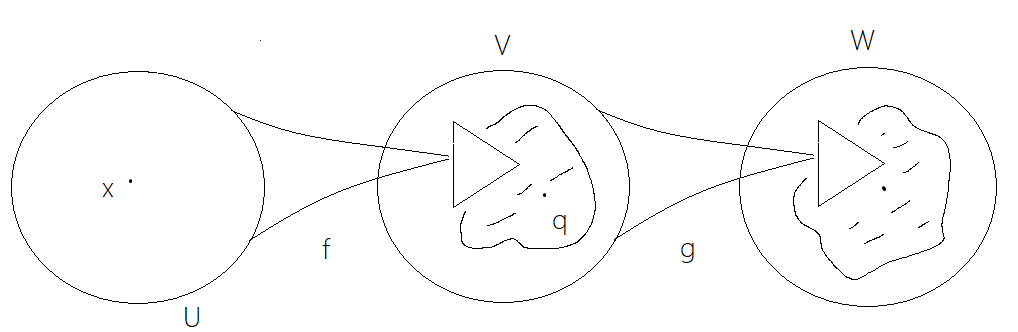
\includegraphics[width=0.8\linewidth]{lect5_1.png}
\end{figure}

\textbf{Доказательство.} Пусть $W$ --- окрестность $(g \circ f)(x) = g(x).$ 

Из того, что $\exists$ окрестность $V \ni y$ т.ч. $g(V) \subset W,$ и $\exists$ окрестность $U \ni x,$ т.ч. $f(U) \subset V,$ следует, что $(g \circ f)(U) \subset W.$ Картинка1 

\textbf{Определение.} $X, Y$ --- топологические пространства, $x \in X, \; f: X \to Y.$ 

$f$ \textbf{секвенциально непрерывно} в $x \; \Leftrightarrow \; \forall$ последовательности $(x_{n})$ в $X,$ т.ч. $x_{n} \to x,$ выполнено $f(x_{n}) \to f(x).$ 

\textbf{Предложение.} $f: X \to Y$ --- отображение топологических пространств, $x \in X.$ 

$(1) \; f$ непрерывна в $x \; \Rightarrow f$ секвенциально непрерывно в $x;$

$(2) \;$ Если $X$ удовлетворяет первой аксиоме счетности (например, метризуемо), то верно и обратное. 

\textbf{Доказательство.} (1) Пусть $x_{n} \to x, \; V$ --- окрестность $f(x).$ 

$\exists$ окрестность $U \ni x$ т.ч. $f(U) \subset V.$ $\exists N \in \mathbb{N}: \; \forall  n \geq N \; x_{n} \in U \; \Rightarrow \forall n \geq N \; f(x_{n}) \in V \; \Rightarrow f(x_{n}) \to f(x).$ 

(2) Предположение: $f$ не является непрерывным в $x.$ 

$\exists$ база окрестностей $\{U_{n}: \; n \in \mathbb{N}\}$ точки $x,$ т.ч. $U_{n} \supset U_{n + 1} \; \forall n;$ 

$\exists$ окрестность $V \ni f(x),$ т.ч. $f(U_{n}) \ni \subset V \; \forall n \in \mathbb{N}.$ 

Т.е. $\forall n \in \mathbb{N} \; \exists x_{n} U_{n},$ т.ч. $f(x_{n}) \ni V \Rightarrow x_{n} \to x,$ но $f(x_{n}) \ni \rightarrow f(x)$ --- противоречие. $\quad \square$ 

\textbf{Обозначение.} $C(X, Y) = \{f: X \to Y | \text{f непрерывно}\}.$ 

$C(X) = C(X, \mathbb{K}),$ где $\mathbb{K} = \mathbb{R}$ или $\mathbb{C}.$

\textbf{Определение.} $f \in C(X, Y)$ --- \textbf{гомеоморфизм} $\Leftrightarrow \exists g \in C(Y, X),$ т.ч. $fg = id_{Y}, \; gf = id_{X}.$ 

\textbf{Определение'} (эквивалентное предыдущему). $f: X \to Y$ --- \textbf{гомеоморфизм} $\Leftrightarrow \; f$ непрерывно и биективно, $f^{-1}$ непрерывно. 

\textbf{Наблюдение.} (1) $f: X \to Y$ --- гомеоморфизм $\Rightarrow f^{-1}: \; Y \to X$ --- гомеоморфизм. 

(2) $f: X \to Y, \; g: Y \to Z$ --- гомеоморфизм $\Rightarrow g \circ g: X \to Z$ --- гомеоморфизм. 

\textbf{Определение.} $X$ и $Y$ \textbf{гомеоморфны} $\Leftrightarrow \; \exists$ гомеоморфизм $X \to Y.$ 

\textbf{Определение.} $X, Y$ --- топологические пространства, $f: X \to Y.$ 

$f$ \textbf{открыто} $\Leftrightarrow \; \forall$ открытых $U \subset X \quad f(U)$ открыто в $Y.$ 

$f$ \textbf{замкнуто} $\Leftrightarrow \; \forall$ замкнутых $B \subset X \quad f(B)$ замкнуто в $Y.$ 

\textbf{Наблюдение.} Отображение $f: X \to Y$ --- гомеоморфизм $\Leftrightarrow f$ непрерывно, биективно и открыто или $\Leftrightarrow \; f: X \to Y$ непрерывно, биективно и замкнуто.

\textbf{Пример-упражнение 1.} $X$ --- нормированное пространство, $x \in X, \; r > 0.$ 

$f: B_{1}(0) \to B_{r}(x), \; f(y) = x + ry$ --- гомеоморфизм. 

\textbf{Пример-упражнение 2.} $X$ --- нормированное пространство. 

$ff: B_{1}(0) \to X, \; f(x) = \dfrac{x}{1 - ||x||}$ --- гомеоморфизм. 

\begin{wrapfigure}{R}{0.3\textwidth}
	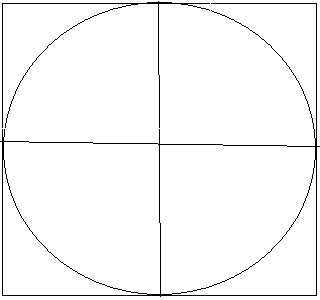
\includegraphics[width=0.7\linewidth]{lect5_2.png}
\end{wrapfigure}

\textbf{Пример-упражнение 3.} $S^{1} = \{(x, y) \in \mathbb{R}^{2}: \; x^{2} + y^{2} = 1\}.$ 

$C = \{(x, y) \in \mathbb{R}^{2}: \max\{|x|, |y|\} = 1\}.$ 

$f: C \to S^{1}, \; f(p) = \dfrac{p}{||p||_{2}}$ --- гомеоморфизм. 

\begin{figure}[htpb]
	\centering
	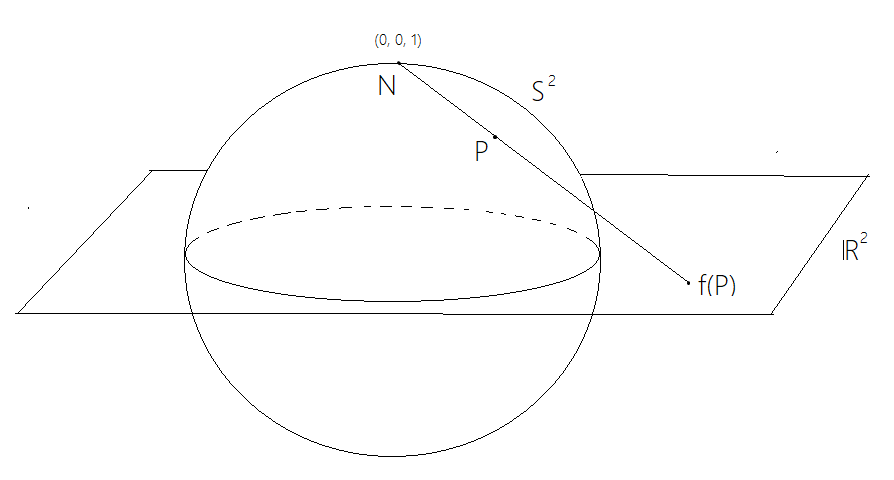
\includegraphics[width=0.8\linewidth]{lect5_3.png}
\end{figure}

\textbf{Пример-упражнение 4} (стереографическая проекция)

$S^{2} = \{(x, y, z) \in \mathbb{R}^{3}: \; x^{2} + y^{2} + z^{2} = 1\}$ --- сфера. 

$f: \; S^{2} \backslash \{N\} \to \mathbb{R}^{2}$ --- гомеоморфизм. 

Упражнение. Построить аналогичный гомеоморфизм между $S^{n} \backslash \{\mathbb{N}\}$ и $\mathbb{R}^{n}.$ 

\textbf{Определение.} Топологическое пространство $M$ --- \textbf{топологическое многообразие ($C^{0}$-многообразие)} размерности $n,$ если 

(1) $M$ хаусдорфово; 

(2) $M$ со счетной базой; 

(3) $\forall x \in M \; \exists$ окрестность $U \ni x,$ гомеоморфная открытому подмножеству в $\mathbb{R}^{n}$ (здесь топология на $U$ определяется так: $V \subset U$ открыто в $U \; \Leftrightarrow V$ открыто в $M$). 

Если $U$ --- как в (3), $\varphi: \; U \to V$ --- гомеоморфизм, где $V \subset \mathbb{R}^{n}$ открыто, то $(U, \varphi)$ называется \textbf{картой} на $M.$ 

\textbf{Пример 1.} $\mathbb{R}^{n}$ --- топологическое многообразие. 

\textbf{Пример-упражнение 2.} Открытое подмножество в $\mathbb{R}^{n}$ --- топологическое многообразие (упражнение: доказать наличие счетной базы). 

\textbf{Пример-упражнение 3.} Сфера $S^{n} \subset \mathbb{R}^{n + 1}, \; S^{n} = \{x \in \mathbb{R}^{n + 1}: \; ||x||_{2} = 1\}$ --- топологическое многообразие. Упражнение: сколькими картами она покрывается? 

\subsection{Подпространства топологических пространств} 

$(x, \tau)$ --- топологическое пространство, $Y \subset X.$ 

\textbf{Обозначение.} $\tau_{Y} = \{V \cap Y: \; U \in \tau\}.$ 

\textbf{Наблюдение.} $\tau_{Y}$ --- топология на $Y.$ 

\textbf{Определение.} $\tau_{Y}$ --- топология, \textbf{индуцированная (унаследованная)} из $(x, \tau).$ $(Y, \tau_{Y})$ называется \textbf{топологическим подпространством} в $(X, \tau).$

\textbf{Предложение.} Пусть $(X, \rho)$ --- метрическое пространство, $Y \subset X, \; \tau_{\rho}$ --- топология на $Y,$ порожденная ограничением метрики $\rho$ на $Y \times Y \Rightarrow \tau_{\rho} = \tau_{Y}.$ 

\textbf{Доказательство.} Базу $\tau_{\rho}$ образуют шары $B_{r}^{Y} = \{z \in Y: \; \rho(z, y) < r\} \; (y \in Y, r > 0).$ 

\textbf{Замечание.} $B_{r}^{Y}(y) = B_{r}(y) \cap Y$ (где $B_{r}(y) = \{z \in X: \; \rho(z, y) < r\}) \Rightarrow B_{r}^{Y} \in \tau_{Y} \Rightarrow \tau_{\rho} \subset \tau_{Y}.$ 

Пусть $V \in \tau_{Y}; \; V = U \cap Y,$ где $U$ открыто в $X.$ 

Пусть $y \in V \Rightarrow \exists r > 0,$ т.ч. $B_{r}(y) \subset U \Rightarrow B_{r}^{Y}(y) \subset V \Rightarrow V \in \tau_{\rho} \Rightarrow \tau_{Y} = \tau_{\rho}. \quad \square$ 

\begin{figure}[htpb]
	\centering
	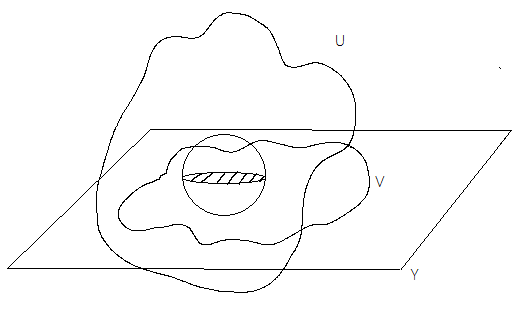
\includegraphics[width=0.6\linewidth]{lect5_4.png}
\end{figure}

\textbf{Обозначение.} $X$ --- множество, $Y \subset X.$ $y_{Y}: Y \to X, \; i_{Y}(y) = y \; \forall y \in Y$ --- \textbf{отображение включения} $Y$ в $X.$ 

\textbf{Теорема} (основные свойства индуцированной топологии)

$(X, \tau)$ --- топологическое пространство, $Y \subset X.$ Снабдим $Y$ индуцированной топологией $\tau_{y}.$ 

(1) $\tau_{Y}$ --- самая грубая топология на $Y,$ в которой $i_{Y}: \; Y \to X$ непрерывно;

(2) Если $Z$ --- топологическое пространство, то $f: Z \to Y$ непрерывно $\Leftrightarrow \; i_{Y} \circ f: Z \to X$ непрерывно. 

Иначе говоря, $f$ непрерывно как отображение из $Z$ в $Y \; \Leftrightarrow$ оно непрерывно как отображение из $Z$ в $X.$ 

\textbf{Доказательство.} (1) $i_{Y}^{-1}(U) = U \cap Y \Rightarrow i_{Y}$ непрерывно. Пусть $\sigma$ --- топология на $Y,$ т.ч. $i_{Y}: (Y, \sigma) \to X$ непрерывно $\Rightarrow \; \forall U \in \tau \; i_{Y}^{-1} (= U \cap Y) \in \sigma \Rightarrow \tau_{Y} \subset \sigma.$ 

(2) $\forall U \subset X \; (i_{Y} \circ f)^{-1}(U) = f^{-1}(i_{Y}(U)) = f^{-1}(U \cap Y).$

$i_{Y} \circ f$ непрерывно $\Leftrightarrow \forall U \in \tau \; (i_{Y} \circ f)^{-1}(U)$ открыто в $Z \Leftrightarrow \forall V \in \tau_{Y} \; f^{-1}(V)$ открыто в $Z$ и $\Leftrightarrow f$ непрерывна. $\square$

\textbf{Упражнение.} $\tau_{Y}$ --- единственная топология на $Y,$ удовлетворяющая (1), и единственная топология на $Y,$ удовлетворяющая (2).

[дальше лекция 21.11.19]

$(X, \tau)$ --- топологическое пространство $Y \subset X.$ 

$\tau_{Y} = \{U \cap Y: \; U \in \tau\}$ --- \textbf{индуцированная топология} на $Y.$ 

$i_{Y}: Y \to X$ --- отображение включения: $i_{Y}(y) = y \quad \forall y \in Y.$

$\tau_{Y}$ --- самая грубая топология на $Y,$ в которой $i_{Y}$ непрерывно. 

\textbf{Определение.} $f: X \to Y$ --- отображение множеств, $A \subset X.$ 

\textbf{Ограничение} $f$ на $A$ --- это $f\backslash_{A}: \; A \to Y, (f\backslash_{A})(a) = f(a) \quad \forall a \in A.$ 

\textbf{Предложение.} $X, Y$ --- топологические пространства, $A \subset X, \; f: X \to Y$ непрерывно $\Rightarrow f \backslash_{A}: A \to Y$ непрерывно. 

\textbf{Доказательство.} $f\backslash_{A} = f \circ i_{A}. \quad \square$

\textbf{Предложение.} (1) Множество $B \subset Y$ замкнуто в $\tau_{Y} \; \Leftrightarrow B = F \cap Y$ для некоторого замкнутого $F \subset X.$ 

$\quad \quad \quad (2) \forall A \subset Y$ (замыкание $A$ в $(Y, \tau_{Y}) = \overline{A} \cap Y,$ где $\overline{A}$ --- замыкание $A$ в $X.$ 

\textbf{Доказательство.} (1) следует из формулы $Y \backslash B = (X \backslash B) \cap Y \; \forall B \subset Y.$ 

$\quad \quad \quad \quad \quad \quad \quad \quad \quad (2)$ (Замыкание $A$ в $Y$) = $\bigcap\{C \subset Y: \; C$ замкнуто в $(Y, \; \tau_{Y})$ и $C \supset A\} \overset{(1)}{=} \bigcap \{F \cap Y: \; F$ замкнуто в $X$ и $F \supset A\} = (\bigcap \{F: F$ замкнуто в $X$ и $F \supset A\}) \cap Y = \overline{A} \cap Y. \quad \square$ 

\textbf{Предложение.} $X$ --- топологическое пространство, $A \subset Y \subset X.$ 

(1) Если $Y$ открыто в $X,$ то $A$ открыто в $Y \; \Leftrightarrow A$ открыто в $X.$

(2) Если $Y$ замкнут в $X,$ то $A$ замкнут в $Y \; \Leftrightarrow A$ замкнут в $X.$

\textbf{Доказательство.} (1) $(\Rightarrow) \; A = Y \cap U,$ где $U$ открыто в $X \Rightarrow A$ открыто в $X.$

$\quad \quad \quad (\Leftarrow) \; A = Y \cap A,$ где $A$ открыто в $X, \; \Rightarrow A$ открыто в $Y.$ 

(2) Аналогично. $\quad \square$ 

\section{Инициальные топологии. Произведения топологических пространств}

\subsection{Инициальные точки} 

$X$ --- множество, $(X_{i}, \tau_{i})_{i \in I}$ --- семейство топологических пространств $(I \neq \varnothing); \; (f_{i}: X \to X_{i})_{i \in I}$ --- семейство отображений.

\textbf{Определение.} \textbf{Инициальная топология на $X,$} порожденная семейством $(f_{i})_{i \in I},$ --- это топология $\tau_{in}$ на $X$ с предбазой $\{f^{-1}_{i}(U): \; i \in I, U \in \tau_{i}\}.$ 

\textbf{Пример 1.} $X$ --- топологическое пространство, $Y \subset X.$

Инициальная топология на $Y$ = инициальная топология, порожденная $\{i_{Y}: \; Y \to X\}.$ 

\textbf{Обозначение.} $pt$ --- топологическое пространство,состоящее из одной точки.

\textbf{Пример 2.} $X$ --- множество. Инициальная топология на $X,$ порожденная $\{X \to pt\},$ --- антидискретная топология. 

\textbf{Теорема (основные свойства инициальной топологии).} $X$ --- множество, снабженное инициальной топологией, порожденной семейством $(f_{i}: \; X \to X_{i})_{i \in I}.$ 

(1) $\tau{in}$ --- самая грубая топология на $X,$ в которой все $f_{i}$ непрерывны; 

(2) Если $Y$ --- топологическое пространство, то отображение $g: \; Y \to X$ непрерывно $\Leftrightarrow f_{i} \circ g: \; Y \to X_{i}$ непрерывно $\forall i.$ 

\begin{wrapfigure}{R}{0.3\textwidth}
	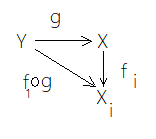
\includegraphics[width = 5cm]{lect6_3.png}
\end{wrapfigure}

\textbf{Доказательство.} (1) $\forall i \in I \; \forall U \in \tau_{i} \quad f_{i}^{-1}(U) \in \tau_{in} \; \Rightarrow f_{i}$ непрерывно.

Пусть $\sigma$ --- некоторая топология на $X,$ т.ч. $\forall i \in I \quad f_{i}: (X, \sigma) \to X_{i}$ непрерывно. 

$\forall i \in I \; \forall U \in \tau_{i} \quad f-{i}^{-1}(U) \in \sigma \; \Rightarrow$ (предбаза $\tau_{in}) \subset \sigma \Rightarrow \tau_{in} \subset \sigma.$ 

(2) $(\Rightarrow)$ Если $g$ непрерывно, то $f_{i} \circ g$ непрерывно, т.к. $f_{i}$ непрерывно. 

$(\Leftarrow)$ Пусть $f_{i} \circ g$ непрерывно $\forall i.$ 

Достаточно доказать: $\forall$ множества $V \subset X$ из предбазы $\tau_{in} \quad g^{-1}(V)$ открыто в $Y.$

$V = f_{i}^{-1}(U),$ где $U \subset X_{i}$ открыто $\Rightarrow g^{-1}(V) = g^{-1}(f_{i}^{-1}(U)) = (f_{i} \circ g)^{-1}(U)$ --- открыто в $Y. \quad \square$ 

\textbf{Упражнение.} $\tau_{in}$ --- единственная топология на $X$ со свойством (2).

\subsection{Произведения множеств} 

$(X_{i})_{i \in I}$ --- семейство множеств. 

\textbf{Определение.} \textbf{Произведение} семейства $(X_{i})_{i \in I}$ --- множество. 

$\underset{i \in I}{\text{П}} = \{x: \; I \to \underset{i \in I}{\bigcup} X_{i} \; | \; \forall i \in I \; x(i) \in X_{i}\}.$ 

\textbf{Частный случай.} Если $X_{i} = Y \quad \forall i,$ то $\underset{i \in I}{\text{П}} X_{i} = Y^{I}$ --- множество всех отображений $I \to Y.$

\textbf{Обозначения.} $\forall x \in \underset{i \in I}{\text{П}} X_{i}, \quad x_{i} = x(i), \quad x = (x_{i})_{i \in I} \; (x_{i} \in X_{i}).$ 

Если $I = \{1, 2, ..., n\},$ то вместо $\underset{i \in I}{\text{П}}X_{i}$ пишут $\overset{n}{\underset{i = 1}{\text{П}}}X_{i}$ или $X_{1} \times X_{2} \times ... \times X_{n}.$ 

В этом случае элементы $X_{1} \times ... \times X_{n}$ --- упорядоченные наборы $(x_{1}, ..., x_{n}),$ где $x_{i} \in X_{i}.$ 

\textbf{Обозначение.} $\forall j \in I \; p_{j}: \underset{i \in I}{\text{П}} X_{i} \to X_{j}, \; p_{j}(x) = x_{j}.$ 

$p_{j}$ --- \textbf{каноническая проекция} на $x_{j}.$ 

\subsection{Произведения топологических пространств} 

$(X_{i}, \tau_{i})_{i \in I}$ --- семейство топологических пространств, $X = \underset{i \in I}{\text{П}} X_{i}.$ 

\textbf{Определение.} \textbf{Топология произведения} (тихоновская топология) на $X$ --- это инициальная топология, порожденная семейством $\{p_{j}: X \to X_{j}\}_{j \in I}\}$ --- канонических проекций.

\textbf{Наблюдение.} (1) $\forall$ открытых $U \in X_{i}$ 

$(*) \; p_{i}^{-1}(U) = \underset{j \in J}{\text{П}} V_{j},$ где $V_{j} = 
\begin{cases}
U &\text{при j = i,}\\
X_{j} &\text{при $j \neq i.$}
\end{cases}$

Множества вида (*) образуют предбазу $X.$ 

(2) $\forall$ конечного $I_{0} \subset I, \; \forall i \in I_{0}$ пусть $U_{i} \subset X_{i}$ --- открытое множество. 

(**) $\underset{i \in I_{0}}{\bigcap} p_{i}^{-1}(U_{i}) = \underset{j \in I}{V_{j}},$ где $V_{j} = 
\begin{cases}
U_{j}, &\text{если $j \in I_{0}$}\\
X_{j}, &\text{если $j \not \in I_{0}$}
\end{cases}$

Множества вида (**) образуют базу $X.$ 

(3) Если $I$ конечно, то базу $X$ образуют множества вида $\underset{i \in I}{U_{i}},$ где $U_{i} \subset X_{i}$ открыто. 

\textbf{Предостережение-упражнение.} Если $I$ бесконечно, то $\underset{i \in I}{\text{П}}U_{i}$ необязательно открыто в $X$ (где $U_{i} \subset X_{i}$ открыто).

\textbf{Отступление.} Коммутативные диаграммы 

\begin{figure}[htpb]
	\centering
	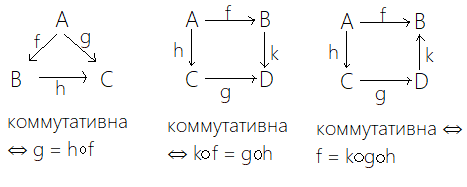
\includegraphics[width=0.8\linewidth]{lect6_1.png}
\end{figure}

\textbf{Теорема (универсальное свойство произведения).} $(x_{i})_{i \in I}$ --- семейство топологических пространств, $X = \underset{i \in i}{\text{П}} X_{i}, \quad p_{i}: X \to X_{i}$ --- каноническая проекция, $Y$ --- топологическое пространство. 

\begin{wrapfigure}{L}{0.3\textwidth}
	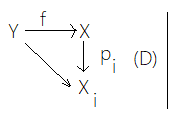
\includegraphics[width = 5cm]{lect6_2.png}
\end{wrapfigure}

Тогда $\forall$ семейства $(f_{i}: Y \to X_{i})_{i \in I}$ непрерывных отображений $\exists !$ непрерывное отображение $f: Y \to X,$ т.ч. диаграмма $(D)$ коммутативна $\forall i \in I.$ 

\textbf{Доказательство.} Определим $f: Y \to X$ так: $(f(y))_{i} = f_{i}(y) \quad \forall y \in Y, \; \forall i \in I.$

Отображение $f$ делает диаграмму $(D)$ коммутативной и является единственным отображением с этим свойством. Его непрерывность следует из теоремы о свойствах инициальной топологии. $\square$ 

\textbf{Предложение.}$(x_{i}, \; \rho_{i}) \; (i = 1, 2, 3, ..., n)$ --- метрическое пространство, $X = \underset{i = 1}{\text{П}} X_{i}.$

Определим $\rho: X \times X \to [0; +\infty)$ так: $\rho(x, y) = \underset{1 \leq i \leq n}{max} \rho_{i}(x_{i}, y_{i}).$ 

Тогда $\rho$ --- метрика на $X,$ и она порождает топологию произведения на $X.$ 

\textbf{Доказательство.} Упражнение. $\rho$ --- метрика. Обозначим $\tau$ = топология на $X,$ $\tau_{\rho}$ --- топология, порожденная $\rho.$ 

\textbf{Заметим:} $\rho(x, y) < r \Leftrightarrow \rho_{i}(x_{i}, y_{i}) < r \quad \forall i = 1, ..., n \quad \Leftrightarrow B_{r}(x) = \overset{n = 1}{\underset{i = 1}{\text{П}}} B_{r}(x_{i}) \Rightarrow B_{r}(x)$ открыт в $\tau \Rightarrow \tau_{\rho} \subset \tau.$

Пусть $U$ --- множество из базы $\tau; \; U = \overset{n}{\underset{i = 1}{\text{П}}} U_{i},$ где $U_{i} \subset X_{i} \; \forall i$ открыто. 

Пусть $x \in U.$ Тогда $\forall i = 1, ..., n \quad x_{i} \in U_{i} \Rightarrow \exists r_{i} > 0$ т.ч. $B_{r_{i}} (x_{i}) \subset \overset{n}{\underset{i = 1}{\text{П}}} U_{i} = U.$ 

$\Rightarrow U$ открыто в $\tau_{\rho} \Rightarrow \tau \subset \tau_{\rho} \Rightarrow \tau = \tau_{\rho}. \quad \square$ 

\textbf{Следствие.} $\mathbb{K} = \mathbb{R}$ или $\mathbb{C}.$ Стандартная топология на $\mathbb{R}^{n},$ порожденная $|| \cdot ||_{\infty}$ (или $|| \cdot ||_{1}, \; || \cdot ||_{2}),$ совпадает с топологией произведения $\mathbb{K} \times ... \times \mathbb{K}.$

\textbf{Доказательство.} Определим $f: Y \to X$ так: $(f(y))_{i} = f_{i}(y) \quad \forall y \in Y \quad \forall i \in I.$ 

Отображение $f$ делает диаграмму (D) коммутативной и является отображением с этим свойством. Его непрерывность следует из теоремы о свойствах инициальной топологии. $\square$

\textbf{Определение.} $(X_{i}, \rho_{i}) \; (i = 1, ..., n)$ --- метрические пространства, $X = \underset{i = 1}{\overset{n}{\text{П}}} X_{i}.$ 

Определим $\rho: \; X \times X \to [0; +\infty]$ так: $\rho(x, y) = \underset{1 \leq i \leq n}{max} \rho_{i} (x_{i}, y_{i}).$ 

Тогда $\rho$ --- метрика на $X,$ и она порождает топологию произведения на $X.$ 

\textbf{Доказательство.} Упражнение. $\rho$ --- метрика. 

Обозначение. $\tau$ = топология произведения на $X, \; \tau_{\rho}$ --- топология, порожденная $\rho.$ Заметим: $\rho(x, y) < r \Rightarrow \rho_{i} (x_{i}, y_{i}) < r \quad \forall i = 1, ..., n \Rightarrow B_{r} (x) = \underset{i = 1}{\overset{n}{\text{П}}} B_{r}(X_{i}) \Rightarrow B_{r} (X)$ открыто в $\tau \; \Rightarrow \tau_{\rho} \subset \tau.$ 

Пусть $U$ --- множество из базы $\tau; \; U = \underset{i = 1}{\overset{n}{\text{П}}} U_{i},$ где $U_{i} \subset X_{i} \quad \forall i$ открыто. 

Пусть $x \in U.$ Тогда $\forall i = 1, ..., b \quad x_{i} \in U_{i} \Rightarrow \exists r_{i} > 0: \; B_{r}(x_{i}) \subset U_{i}.$ 

Обозначим $r = \underset{1 \leq i \leq n}{\min} r_{i} \Rightarrow B_{r}(x) = \underset{i = 1}{\overset{n}{\text{П}}} B_{r} (x_{i}) \subset \underset{i = 1}{\overset{n}{\text{П}}} B_{r_{i}} (x_{i}) \subset \underset{i = 1}{\overset{n}{\text{П}}} U_{i} = U \Rightarrow U$ открыто в $\tau_{\rho} \Rightarrow \tau \subset \tau_{\rho} \Rightarrow \tau = \tau_{\rho}. \quad \square$ 

\textbf{Следствия.} Стандартная топология на $\mathbb{K}^{n},$ порожденная $|| \cdot ||_{\infty}$ (или $|| \cdot||_{1}, \; || \cdot ||_{2}),$ где $\mathbb{K} = \mathbb{R}$ или $\mathbb{C},$ совпадает с топологией произведения $\mathbb{K} \times ... \times \mathbb{K}.$ 

$X$ --- множество, $(X_{i})_{i \in I}$ --- топологические пространства, $(f_{i}: X \to X_{i})_{i \in I}.$ 

$\{f_{i}^{-1}(U)\!: U \subset X_{i}$ открыто, $i \in I$\} является предбазой инициальной топологии $\tau_{in},$ порожденной $(f_{i}).$ 

$(X_{i})_{i \in I}, \; (Y_{i})_{i \in I}$ --- семейства множеств, $f_{i}: \; (X_{i} \to Y_{i})_{i \in I}$ --- семейство отображений. 

\textbf{Определение.} Декартово произведение семейства $(f_{i})$ --- отображение $\underset{i \in I}{\text{П}} f_{i}: \; \underset{i \in I}{\text{П}} X_{i} \to \underset{i \in I}{\text{П}} Y_{i}. \quad (X_{i})_{i \in I} \to (f_{i}(X_{i}))_{i \in I}.$

\textbf{Предположение.} Пусть $(X_{i})_{i \in I}, (Y_{i})_{i \in I}$ --- семейства топологических пространств, $f_{i}: X_{i} \to Y_{i})_{i \in I}$ --- семейство непрерывных отображений $\Rightarrow \text{П} f_{i}: \text{П} X_{i} \to \text{П} Y_{i}$ непрерывно. 

\textbf{Доказательство.} П$X_{i} = X, \; \text{П}Y_{i} = Y \; \text{П} f_{i} = f.$

\begin{wrapfigure}{R}{0.3\textwidth}
	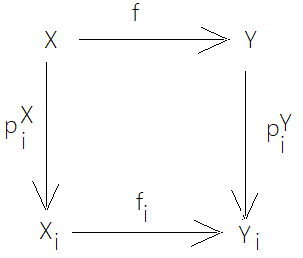
\includegraphics[width = 5cm]{lect7_1.png}
\end{wrapfigure}

$f$ непрерывно $\Leftrightarrow \; p_{i}^{Y} \circ f$ непрерывно $\forall i$ (см. свойства инициальной топологии) $\Leftrightarrow f_{i} \circ p_{i}^{X}$ непрерывно, а это верно по условию. $\square$ 

\textbf{Следствие.} $X$ --- топологическое пространство. $\mathbb{K} = \mathbb{R}$ или $\mathbb{C}, \; C(X) = C(X, \mathbb{R}).$

Тогда $\forall f, \; g \in C(X) \; f + g \in C(X)$ и $fg \in C(X).$ Если $f(x) \neq 0 \quad \forall x \in X \Rightarrow \dfrac{1}{f} \in C(X).$ 

$X \underset{x \underset{\text{непрерывно}}{\mapsto} (x, x)}{\overset{\Delta}{-\!\!\!-\!\!\!-\!\!\!-\!\!\!-\!\!\!\to}}X \times X \underset{\text{непрерывно}}{\overset{f \times g}{-\!\!\!-\!\!\!-\!\!\!-\!\!\!-\!\!\!\to}} \mathbb{K} \times \mathbb{K} \underset{\text{непрерывно}}{\overset{+}{-\!\!\!-\!\!\!-\!\!\!-\!\!\!-\!\!\!\to}} \mathbb{K},$ т.е. $X \overset{f + g}{-\!\!\!-\!\!\!-\!\!\!-\!\!\!-\!\!\!\to} \mathbb{K}, \; \Rightarrow f + g$ непрерывно. Аналогично $fg$ непрерывно. 

$X \underset{\text{непрерывно}}{\overset{f}{-\!-\!\to}} \mathbb{K} \backslash \{0\} \underset{\text{непрерывно}}{\overset{t \mapsto \dfrac{1}{t}}{-\!-\!\to}},$ т.е. $X \overset{\dfrac{1}{t}}{\to} \mathbb{K} \Rightarrow \dfrac{1}{f}$ непрерывно. $\square$ 

\textbf{Предложение.} Топологическое пространство $X$ хаусдорфово $\Leftrightarrow$ диагональ $D_{x} = \{(x, \; x): \; x \in X\} \subset X \times X$ замкнута в $X \times X.$ 

\begin{wrapfigure}{R}{0.3\textwidth}
	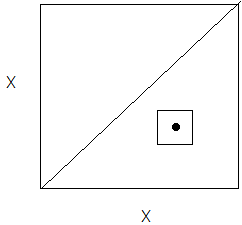
\includegraphics[width = 5cm]{lect7_2.png}
\end{wrapfigure}

\textbf{Доказательство.} $D_{X}$ замкнута в $X \times X \; \Leftrightarrow \forall p \in (X \times X) \backslash D_{X} \; \exists$ окрестность $W \ni p$ вида $W = U \times V,$ где $U, V$ --- открыто в $X,$ т.ч. $W \cap D_{x} = \varnothing.$ 

$\Leftrightarrow \forall x, y \in X,$ т.ч. $x \neq y \; \exists$ открытые $U, V \subset X,$ т.ч. $x \in U, y \in V$ и $U \cap V = \varnothing \Leftrightarrow X$ --- хаусдорфово. $\square$ 

\textbf{Следствие 1. Предложение.} $X, Y$ --- топологические пространства, $Y$ --- хаусдорфово, $f, g: X \to Y$ непрерывно $\Rightarrow \; \{x \in X: \; f(x) = g(x)\}$ замкнуто в $X.$

\textbf{Доказательство.} $F: \; X \to Y \times Y, \; F(x) = (f(x), g(x))  \; F$ непрерывно, $\{x: \; f(x) = g(x)\} = F^{-1}(D_{Y}),$ а $D_{Y}$ замкнуто в $Y \times Y. \quad \square$

\textbf{Следствие 2.} $X, Y$ --- топологические пространства, $Y$ --- хаусдорфово, $f, g: X \to Y$ непрерывно. Пусть $X_{0} \subset X$ --- плотное подмножество, т.е. замыкание содержит все пространство, $f \backslash_{X_{0}} = g \backslash_{X_{0}} \Rightarrow f = g.$ 

\textbf{Доказательство.} Множество $S = \{x \in X: f(x) = g(x)\}$ замкнуто и содержит $X_{0} \; \Rightarrow S = X. \quad \square$

\section{Финальные топологии и дизъюнктные объединения}

\subsection{Финальные топологии}

$X$ --- множество, $(X_{i}, \tau_{i})_{i \in I}$ --- семейство топологических пространств. $(f_{i}: X_{i} \to X)_{i \in I}$ --- семейство отображений.

\textbf{Определение.} \textbf{Финальная топология} на $X,$ порожденная $(f_{i})_{i \in I}$ --- это $\tau_{f_{i \not \in I}} = \{U \subset X: f_{i}^{-1}(U) \in \tau_{i} \quad \forall i \in I\}.$

\textbf{Замечание.} $\tau_{f_{in}}$ является топологией на $X.$

\textbf{Предложение.} Финальная топология на $X,$ порожденная отображением $\{\varnothing \to X\},$ --- дискретная топология. 

\textbf{Теорема 1 (основное свойство финальной топологии)}

(1) $\tau_{f_{in}}$ --- самая тонкая топология на $X,$ т.ч. все $f_{i}: \; X_{i} \to X$ непрерывны. 

(2) Если $Y$ --- топологическое пространство, то отображение $g: \; X \to Y$ непрерывно $\Leftrightarrow \; g \circ f_{i}$ непрерывно $\forall i.$ 

\textbf{Доказательство.} (1) $\forall i ]in I \quad \forall U \subset \tau_{f_{in}} \quad f_{i}^{-1} \in \tau_{i}$ --- верно по определению $\tau_{f_{in}} \Rightarrow f_{i}^{-1}$(открытое) = открытое $\Rightarrow f_{i}$ непрерывно. 

Пусть $\sigma$ --- топология на $X,$ т.ч. $\forall i \in I \quad f_{i}: X_{i} \to (X, \sigma)$ непрерывно $\forall U \in \sigma \quad \forall i \in I \quad f^{-1}_{i}(U) \in \tau_{i} \Rightarrow U \in \tau_{fin} \Rightarrow \sigma \subset \tau_{fin}.$ 

(2) $g$ непрерывно $\Leftrightarrow \forall V \subset Y$ открыто, $g^{-1}(V) \in \tau_{fin} \Leftrightarrow \forall$ открытого $V \subset Y \quad \forall i \in I, \quad f_{i}^{-1}(g^{-1}(V)) = (g \circ f_{i})^{-1}(V) \in \tau_{i}.$ 

Упражнение. $\tau_{fin}$ --- топология на $X,$ обладающая свойством (2).

\subsection{Дизъюнктное объединение множеств}

$(X_{i})_{i \in I}$ --- семейство множеств. 

\textbf{Определение.} \textbf{Дизъюнктное объединение} семейства $(X_{i})_{i \in I}$ --- множество $\underset{i \in I}{\sqcup} X_{i} = \{(x, i): i \in I, x \in X_{i}\}.$ 

\textbf{Обозначение}. $\forall j \in I \quad q_{j}: X_{j} \to \underset{i \in I}{\sqcup} X_{i}, \; q_{j}(X) = (X, j)$ --- каноническое вложение $X_{j}$ в $\underset{i \in I}{\sqcup} X_{i}.$ 

\textbf{Наблюдение.} (1) $q_{j}$ --- инъекция $\forall j;$ 

(2) $q_{i} (X_{i}) \cap q_{j}(X_{j}) = 0 \quad \forall i \neq j;$

(3) $\underset{i \in I}{\sqcup} X_{i} = \underset{i \in I}{q_{i}} (X_{i}).$

\textbf{Соглашение.} Отождествляем $X_{j}$ c $q_{j}(X)$ посредством $q_{j}.$

\subsection{Дизъюнктное объединение} топологических пространств (несвязные суммы)

$(X_{i})_{i \in I}$ --- семейство топологических пространств, $X = \underset{i \in I}{\sqcup} X_{i}, \; q_{j}: X_{j} \to X.$

\textbf{Определение.} \textbf{Топология дизъюнктного объединения} на $X$ --- финальная топология, порожденная семейством $(q_{i}: X_{i} \to X)_{i \in I}$ канонических вложений.

Таким образом, $U \subset X$ открыто $\Leftrightarrow U \cap X_{i}$ открыто в $X_{i} \quad \forall i \in I.$ 

\textbf{Теорема 2 (универсальное свойство дизъюнктных объединений)}

$(x_{i})_{i \in I}$ --- семейство топологических пространств, $Y$ --- топологическое пространство, $X = \underset{i \in I}{\sqcup} X_{i}.$ 

Тогда $\forall$ семейства непрерывных отображений $(f_{i}: X_{i} \to Y)_{i \in I} \; \exists !$ непрерывное $f: X \to Y,$ т.ч. диаграмма $(D)$ коммутативна $\forall i \in I.$ 

\begin{wrapfigure}{R}{0.3\textwidth}
	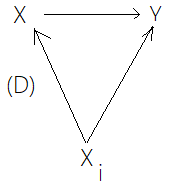
\includegraphics[width = 5cm]{lect7_3.png}
\end{wrapfigure}

\textbf{Доказательство.} Зададим $f: X \to Y$ так: $f((x, i)) = f_{i}(x) \quad (\forall i \in I, \l \forall x \in X_{i}). (*)$

Отображение $f$ делает $(D)$ коммутативной и является единственным отображеним с этим свойством (т.к. (*) эквивалетно $f(q_{i}(x)) = f_{i}(x)$). Непрерывность $f$ --- из теоремы 1. $\square$ 

\section{Связные топологические пространства} 

\textbf{Определение.} Топологическое пространство $X$ \textbf{связно} $\Leftrightarrow \; X$ непредставимо в виде $X = U \cup V,$ где $U, V$ открыто, непусто, $U \cap V = \varnothing.$ 

$X$ \textbf{несвязно} $\Leftrightarrow$ оно связно как топологическое пространство в индуцированной топологии.

\textbf{Наблюдение.} $X$ связано $\Leftrightarrow X$ непредставимо в виде $X = A \cup B,$ где $A, B$ замкнуты, непусты, $A \cap B = \varnothing \; \Leftrightarrow \not \exists$ подмножества $A \subset X, \; A \neq X, A \neq \varnothing,$ открыто и замкнуто одновременно. 

\textbf{Пример.} Дискретное пространство, состоящее более чем из 1 точки, несвязно. 

\textbf{Пример.} Антидискретное пространство связно. 

\textbf{Пример.} $\mathbb{R} \backslash \{0\}$ несвязно, т.к. $\mathbb{R} \backslash \{0\} = (-\infty, 0) \cup (0, +\infty).$ 

\begin{wrapfigure}{R}{0.3\textwidth}
	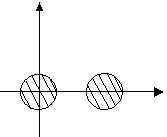
\includegraphics[width = 5cm]{lect7_4.png}
\end{wrapfigure}

\textbf{Пример.} $\overline{B_{1}}(0, 0) \cup \overline{B_{1}}(0, 3) \subset \mathbb{R}^{2}$ --- несвязное.

\textbf{Пример.} $X, Y$ --- непустые топологические пространства $\Rightarrow X \sqcup Y$ несвязно (т.к. X, Y открыты в $X \sqcup Y).$

\textbf{Пример.} $\forall A \subset \mathbb{Q}$ (с топологией, индуцированной из $\mathbb{R}),$ состоящего более чем из одной точки, несвязно.

$a, \; b \in A, \; a  < b \quad \exists$ иррациональное $c \in \mathbb{R}: \; a < c < b.$ 

$\bigcup = A \cap (-\infty, c), \quad V = A \cap (c, +\infty) \Rightarrow U, V$ открыто в $A, \; U \cap V = \varnothing$ и $U \cup V = A.$

\textbf{Предложение.} Отрезок $[a, b] \subset \mathbb{R}$ связен.

\textbf{Доказательство.} Предположим, $[a, b] = U \cup V, \quad U, V \subset [a, b]$ открыты в топологии отрезка $[a, b]),$ непусты, $U \cap V = \varnothing.$

Можем считать: $b \in V \Rightarrow \exists \varepsilon > 0,$ т.ч. $(b - \varepsilon, b] \subset V. \quad (1)$ 

\begin{wrapfigure}{R}{0.4\textwidth}
	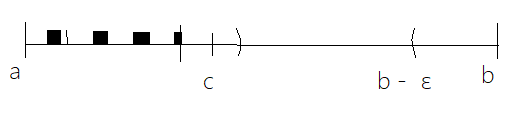
\includegraphics[width=1\linewidth]{lect8_1.png}
\end{wrapfigure}

Обозначим $c = \sup U.$ Заметим: $c > a$ (иначе бы $U = \{a\}$ --- противоречие), $c < b$ в силу (1). 

Если $c \in U \Rightarrow \exists \delta > 0,$ т.ч. $(c - \delta, c + \delta) \subset U \Rightarrow c + \dfrac{\delta}{2} \in U$ --- противоречие с определением $c.$

Если $c \in V \Rightarrow \exists \delta > 0,$ т.ч. $(c - \delta, c + \delta) \subset V \Rightarrow \forall x \in U \quad x \leq c - \delta$ --- противоречие с определением $c \Rightarrow c \not \in U \cup V = [a, b]$ --- противоречие $\Rightarrow [a, b]$ связен. $\square$ 

\subsection{Свойства связных пространств}

\textbf{Теорема (свойства связных пространств)}

(1) $X, Y$ --- топологические пространства, $X$ связно, $f: X \to Y$ непрерывно $\Rightarrow f(X)$ связно. 

(2) Пусть $X = U \cup V, \; U, V$ открыто, $U \cap v = \varnothing;$ пусть $A \subset X$ связно $\Rightarrow A \subset U$ либо $A \subset V.$ 

(3) $A, B \subset X, \; A \subset B \subset \overline{A},$ $A$ связно $\Rightarrow B$ связно.

(4) Пусть $(A_{i})_{i \in I}$ --- семейство связных подмножеств $X,$ имеющих общую точку $\Rightarrow \underset{i \in I}{A_{i}}$ связно.

(5) Пусть любые $x, y \in X$ лежат в некотором связном подмножестве $X \Rightarrow X$ связно. 

(6) $X_{1}, ..., X_{n}$ --- связные топологические пространства $\Rightarrow X_{1} \times ... \times X_{n}$ связно.

\textbf{Доказательство.} (1) Можем считать: $f(X) = Y.$ Пусть $Y = U \cup V, \; U, V \subset Y$ открыты, непусты, $U \cap V = \varnothing.$ 

$f$ --- сюръекция $\Rightarrow X = f^{-1}(U) \cup f^{-1}(V),$ где $f^{-1}(U), \;  f^{-1}(V)$ открыты, непусты, не пересекаются, --- противоречие. 

(2) $A = (U \cap A) \cup (V \cap A) \Rightarrow U \cap A$ либо $V \cap A$ пусто. Если $U \cap A = \varnothing \Rightarrow A = V \cap A,$ т.е. $A \subset V,$ где $U \cap A, \; V \cap A$ открыты в $A$ и не пересекаются. 

(3) Можем считать: $B = X,$ тогда $\overline{A} = X.$ Пусть $X = U \cup V, \; U, V \subset X$ открыты, непусты, $U \cap V = \varnothing.$

Из (2): $A \subset U$ либо $A \subset V.$ Пусть $A \subset U \Rightarrow A \cap V = \varnothing$ --- противоречие с тем, что $\overline{A} = X \Rightarrow X$ связно.

(4) Можем считать: $\underset{i \in I}{\bigcup} A_{i} = X.$ Пусть $a \in A_{i} \quad \forall i \in I.$ 

Пусть $X = U \cap V, \quad U, V \subset X$ открыты, непусты, $U \cap V = \varnothing.$ 

Пусть $a \in U.$ Из (2): $A_{i} \subset U \quad \forall i \in I \Rightarrow V = \varnothing$ --- противоречие $\Rightarrow X$ связно.

(5) Зафиксируем $\forall x \in X.$ 

$\forall y \in X \quad \exists$ связное $A_{xy} \subset X,$ т.ч. $x, y \in A_{xy} \Rightarrow \underset{y \in X}{\bigcup} A_{xy} = X.$ Из (4) $X$ связно.

(6) Достаточно доказать для $n = 2$ (индукция). Обозначим $X_{1} = X, X_{2} = Y.$ Зафиксируем $p = (x_{1}, y_{1}) \in X \times Y, \; q = (x_{2}, y_{2}) \in X \times Y.$ 

Обозначим $A = \{x_{1}\} \times Y, \; B = X \times \{y_{2}\}.$ $A$ гомеоморфно $Y, \; B$ гомеоморфно $X \Rightarrow A, B$ связно. 

$(x_{1}, y_{2}) \in A \cap B \Rightarrow A \cap B = \varnothing \underset{(4)}{--\!\!\to} A \cup B$ связно. 

$p, q \in A \cup B \underset{5}{\Rightarrow} X \to Y$ связно. $\square$ 

\begin{wrapfigure}{R}{0.4\textwidth}
	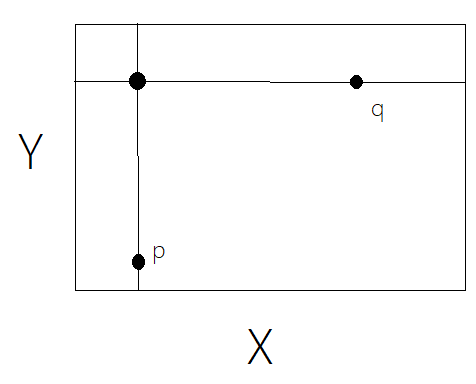
\includegraphics[width=0.9\linewidth]{lect8_2.png}
\end{wrapfigure}

\textbf{Упражнение.} Доказать: произведение $\forall$ семейства топологических пространств связно. 

\textbf{Определение.} $X$ --- топологическое пространство, $x, y \in X.$ \textbf{Пусть} в $X$ из $x$ в $y$ --- непрерывное отображение $f: \; [0, 1] \to X,$ т.ч. $f(0) = x, f(1) = y.$

\begin{wrapfigure}{R}{0.4\textwidth}
	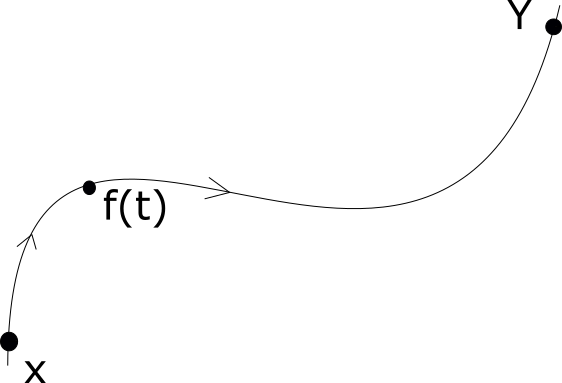
\includegraphics[width=0.8\linewidth]{lect8_3.png}
\end{wrapfigure}

\subsection{Линейно связные пространства}

\textbf{Определение.} $X$ \textbf{линейно связно,} если $\forall x, y \in X \quad \exists$ путь из $x$ в $y.$ 

\textbf{Предложение.} $X$ линейно связно $\Rightarrow X$ связно.

\textbf{Доказательство.} Пусть $x, y \in X, \; f: [0, 1] \to X$ --- пусть из $x$ в $y, \; C = f([0, 1]).$

$C$ связно (т.к. [0, 1] связен, см. пункт (1) теоремы), $x, y \in C.$ Теорема, п. (5) $\Rightarrow X$ связно. $\square$ 

\textbf{Теорема (свойства линейно связных пространств)}

(1) $X, Y$ --- топологические пространства, $X$ линейно связно, $f: X \to Y$ непрерывно $\Rightarrow f(X)$ линейно связно;

(2) $(A_{i})_{i \in I}$ --- семейство линейно связных подмножеств в $X,$ имеющих общую точку $\Rightarrow \underset{i \in I}{\bigcup} A_{i}$ линейно связно; 

(3) $X_{1}, ..., X_{n}$ линейно связны $\Rightarrow X_{1} \times ... \times X_{n}$ линейно связны. 

\begin{wrapfigure}{R}{0.4\textwidth}
	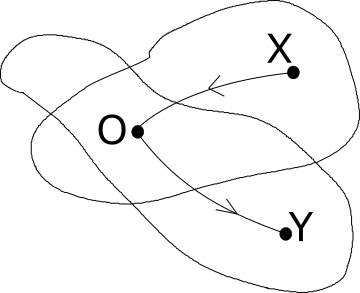
\includegraphics[width=0.8\linewidth]{lect8_4.png}
	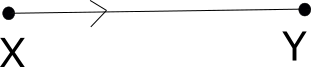
\includegraphics[width=0.8\linewidth]{lect8_5.png}
\end{wrapfigure}

\textbf{Доказательство.} Упражнение. Подсказка к (2) --- рисунок.

\textbf{Пример 1.} $X$ --- нормированное пространство над $\mathbb{R} \Rightarrow X$ линейно связно. 

Действительно: $\forall x, y \in X$ рассмотрим $f: [0, 1] \to X, \; f(t) = ty + (1 - t)x.$ $f$ непрерывно (упражнение), $f(0) = x, \; f(1) = y.$

\textbf{Определение.} Пусть $X$ --- векторное пространство над $\mathbb{R}, \quad x, y \in X.$ Обозначим $[x, y] = \{ty + (1 - t)x: \; 0 \leq t  \leq 1\}.$ Это множество называется \textbf{отрезком} с концами $x, y.$ 

Множество $A \subset X$ \textbf{выпукло} $\Leftrightarrow \quad \forall x, y \in A$ выполнено $[x, y] \subset A.$ 

\begin{wrapfigure}{R}{0.4\textwidth}
	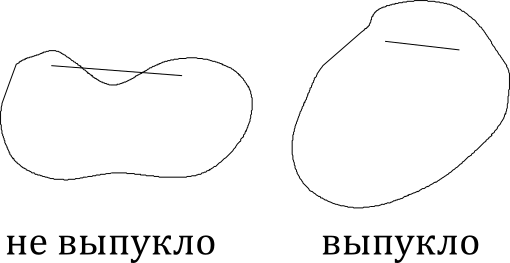
\includegraphics[width=0.8\linewidth]{lect8_6.png}
\end{wrapfigure}

\textbf{Упражнение.} Шар в нормированном пространстве --- выпуклое множество. 

\textbf{Пример 2.} $\forall$ выпуклое подмножество нормированного пространства (над $\mathbb{R})$ линейно связно. Доказательство --- см. пример 1. 

\textbf{Пример-упражнение 3.} $X$ --- нормированное пространство над $\mathbb{R}, \; dim X > 1 \Rightarrow X \backslash \{0\}$ линейно связно. 

\textbf{Пример 4.} $X$ --- нормированное пространство над $\mathbb{R}, \; dim X > 1.$ Сфера $S = \{x \in X: ||x|| =  1\}$ линейно связна. 

\begin{wrapfigure}{R}{0.4\textwidth}
	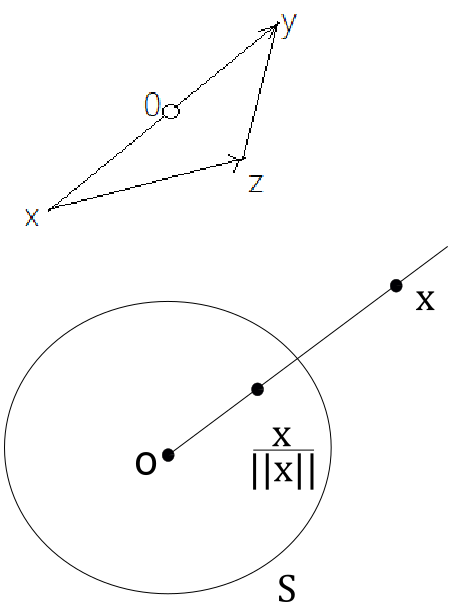
\includegraphics[width=0.8\linewidth]{lect8_78.png}
\end{wrapfigure}

Действительно: рассмотрим $f: \; X \backslash \{0\} \to S, \; f(x) = \dfrac{x}{||x||}.$ (еще рисунок)

\textbf{Пример 5 ($n$-мерный тор).} Обозначим $S^{1} = \{(x, y) \in \mathbb{R}^{2}: x^{2} + y^{2} = 1\}$ (окружность).

$T^{n} = S^{1} \times ... \times S^{1}$ ($n$ раз) --- $n$-мерный тор. $T^{n}$ линейно связно.

\begin{wrapfigure}{R}{0.3\textwidth}
	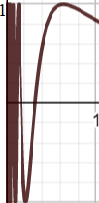
\includegraphics[width=0.8\linewidth]{lect8_9.png}
	\\ \; \\
	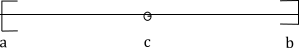
\includegraphics[width=0.8\linewidth]{lect8_10.png}
\end{wrapfigure}

\textbf{Упражнение.} Обозначим $X = \{(x, sin\dfrac{1}{x}): \; 0 < x \leq 1\} \cup \{(0, y): \; -1 \leq y \leq 1\} \subset \mathbb{R}^{2}.$ 

Доказать: $X$ связно, но не линейно связно. 

\textbf{Определение.} Подмножество $A \subset \mathbb{R}$ --- промежуток $\Leftrightarrow A = (a, b),$ где $-\infty \leq a < b \leq +\infty),$ либо $A = [a, b] \; (-\infty < a \leq b < +\infty),$ либо $A = [a, b),$ где $(-\infty < a < b \leq +\infty),$ либо $A = (a, b] \; (-\infty \leq a < b < +\infty),$ либо $A = \varnothing.$ 

\textbf{Упражнение.} $A$ --- промежуток $\Leftrightarrow A$ выпукло.

\textbf{Предложение.} Следующие свойства подмножества $A \subset \mathbb{R}$ эквивалентны:

(1) $A$ связно, (2) $A$ линейно связно, (3) $A$ --- промежуток. 

\textbf{Доказательство.} $(3) \Rightarrow (2)$ --- очевидно, $(2) \Rightarrow (1)$ --- знаем. 

$(1) \Rightarrow (3):$ предположим, что $A$ ограничено. Обозначим $a = inf A, \; b = sup A. \Rightarrow A \subset [a, b].$

Покажем: $(a, b) \subset A.$ (Этого нам достаточно)

Пусть $\exists c \in (a, b),$ т.ч. $c \not \in A.$ Обозначим $U = (-\infty, c) \cap A, \; V = (c, +\infty) \cap A.$

$U, V$ открыты в $A$, $U \cap V = \varnothing,\quad U \cup V = A, \; U \neq \varnothing, \; V \neq \varnothing$ --- противоречие со связностью $A$.

Для неограниченного $A$ рассуждения аналогичны (упражнение). $\square$

\textbf{Следствие (теорема о промежуточном значении)}

$X$ --- связное топологическое пространство, $f \in C(X, \mathbb{R}), \quad x, y \in X \;\; f(x) \leq f(y).$

Тогда $\forall c \in [f(x), f(y)] \; \exists z \in X,$ т.ч. $c = f(z).$

\textit{Доказательство.} $f(X)$ --- связное подмножество $\mathbb{R} \Rightarrow f(X)$ --- промежуток; $f(x), f(y) \in f(X) \Rightarrow [f(x), f(y)] \subset f(X). \quad \square$

\end{document}